\documentclass[11pt,a4paper]{article}

% *** r1839 (PHASE 8, the quadric bake, probe Q1): rem:onecircle / |-58 EXTENDED to the projective
%   setting. The bound was stated for CLASSICAL CIRCLE GEOMETRY in the projection; the polarity of the
%   EMBEDDING QUADRIC itself returns, at every named point, what eq:powerisheight already gives -- because
%   that identity IS the hyperboloid's equation. THE HINGES LIE ON THE QUADRIC (-3+4=1), so each polar is
%   just the tangent hyperplane there, and the sqrt3.alpha tangent length from the foot of the hinge axis
%   is eq:powerisheight at transverse 2alpha, NOT a new relation. Receipt Q1_quadric_polarity.
%   THE FIELD'S TRAP, recorded in QUADRIC_GEOMETRY_LEDGER: a first pass computed the polar's EUCLIDEAN
%   distance in a Minkowski space (1/sqrt7) -- a gauge artefact. Projective quadric geometry's classical
%   formulae are written for Euclidean/complex-projective settings; every length it offers must be checked
%   for invariance under the substrate's own group before it is read as a result. ***
% *** r1847 (PHASE 8, the quadric bake, probe Q3): THE ONE SCALE HAS A CLASSICAL NAME.
%   Read projectively the substrate is a CAYLEY-KLEIN geometry whose ABSOLUTE is the quadric
%   eta(X,X)=0 -- the null cone -- and its geodesic separation IS the CK log-cross-ratio against
%   that absolute, with CK constant = alpha EXACTLY (timelike tau = (alpha/2)|log CR|, verified at
%   every rapidity and every alpha; spacelike the corresponding angle; discriminant 4.alpha^4(u^2-1)
%   in u = eta(P,Q)/alpha^2 deciding which). Receipt Q3_cayley_klein.
%   WHY IT MATTERS: the SCALE is the only free constant a CK construction carries -- signature, null
%   structure and isometry group are fixed by the absolute's projective type -- so ONE SCALE is not
%   merely the outcome of the constants audit (the adversarial hunt's 'audited exhaustive zero') but
%   THE CLASSICAL STATEMENT about a geometry of this kind. The corpus reached it by exhaustion;
%   Cayley-Klein says it structurally.  TRACED, not computed: the only-free-constant fact is
%   standard CK theory. ***
% [†ONT-CORE] THE GEOMETRIC CORE — this paper is the HOME (ONTOLOGY_FOUNDATION_INDEX.md §1j).
%   THE SYNTHESIS POLE (with P7), and the space the corpus lands in. Established here: the substrate is
%   EVERYWHERE INTRINSICALLY REAL BY CONSTRUCTION — a real manifold with a real coordinate basis, its
%   Lorentzian signature intrinsic to its positive curvature; the imaginaries used to REACH it (the
%   fifth embedding coordinate, the conjugacy circle, the seam's continuation) are instruments landing
%   on real points, and the would-be timelike embedding coordinate is NOT a coordinate of the manifold.
%   prop:unique — de Sitter is THE maximally symmetric intrinsically-Lorentzian manifold. The substrate
%   is the UNIVERSAL STANDARD (alpha and the locked null cone the intrinsic length and causal structure;
%   Eddington corrected and grounded; the HORIZON PROBLEM DISSOLVED — the CMB's uniformity is the
%   substrate's maximal symmetry, not early causal contact). The straight null rulings are the light
%   cone: signature and curvature are the asymptote and waist of ONE equilateral pseudo-sphere.
%   *** MAXIMAL SYMMETRY WORN SEVEN WAYS (SO(5,1) complete and exhausted, one root of seven separately-
%   established results): (i) the augmentation necessary and sufficient, its necessary half MEASURED —
%   maximal symmetry making the substrate the LEAST-ARBITRARY vacuum, so the substrate's selection is an
%   instance of the programme's own R2 ([†ONT-EPI]), not an added axiom; (ii) GR's Dirac algebra IS the
%   symmetric-space grading, the problem of time its base-dependence ([†ONT-ALG]); (iii) ONE SCALE — the
%   constants are unit gauges, the grav-cosmo-quantum sector spending NO free dimensionless constant;
%   (iv) the cosmology PARAMETER-FREE ([†ONT-COSMO]); (v) the continuous matter symmetry WALLED
%   (su(3) not in so(5,1) precisely BECAUSE SO(5,1) is exhausted) — but the complement is not empty: the
%   unique spin structure and the one orientation parity acting as gamma^5 ([†ONT-DISC]); (vi) ONE CIRCLE -- the equator/waist is
%   what the construction is built on: its radius IS the curvature, its tangents ARE the null rulings,
%   the power of a point with respect to it is that point's HEIGHT, and P3's hinge placement, 60deg
%   subtense, incircle and nine-point relations all read off it -- P3 calls it "the SEVENTH FACE of the
%   substrate's maximal symmetry".  [COUNT CORRECTED r1883: this header read SIX and enumerated (i)-(vi)
%   while sec:unification enumerates SEVEN and the ALTITUDE line below already said seven. The seventh
%   face was added to the section and the masthead's count was not -- the multi-face indexing defect, in
%   the corpus's own flagship instance.]  (vii) the
%   UNIVERSALITY of physics IS the maximal symmetry (invariance of the measure).
%   THE RIGIDITY AND THE WALL ARE ONE FACT: what makes CR decisive against the world (no knob at any
%   rung) is what makes matter geometrically hard. "The discrete half of matter is the stone's and the
%   content half the search." LEDGER: the Planck values are gauge-combinations, not physical scales;
%   alpha is the one physical length; alpha/l_P ~ 10^61 is a NUMBER, NOT A TUNING; Lambda's VALUE is the
%   ledger's one input, NOT predicted. ***
%   *** ALTITUDE (P6's boundary, enacted — hold this): the seven results are EACH ESTABLISHED; reading
%   them as ONE FACT is the THESIS, tagged [reach], decidable by the test in §frontiers. The
%   two-fine-tuning-problems-one-fact reading is CONJECTURE. Assert neither a geometric su(3), nor the
%   hexad IDENTITY (the geometric six-fold and the flavour triplet are two distinct O(5,1) reflections
%   — R vs T, a true resonance, NOT a naming-blocker: R carries 3->3bar, so the R-image branch is
%   antimatter within CR at the weight the fundamental is matter), and a geometric CPT is not
%   auto-yielded (the residue is a LINEAR orientation skeleton P/T/gamma^5/R; charge conjugation is
%   antilinear and field-level — the geometry supplies the orientation SKELETON of matter AND antimatter,
%   the 3(+)3bar the R-parity relates, not the CHARGE, which is field-level on both branches alike), nor
%   the generation descent's world-correspondence. COHERENCE, NOT CORRESPONDENCE. ***
%   *** UPDATE (r1088->r1092): "field-level" enlarged. The antilinear structure is NOT wholly field-level:
%   tau~ -> conj(tau~) is antilinear AND geometric (L2), so C FACTORISES, C = (Q->-Q)_field o (R o K)_geom,
%   the geometry carrying all of C's KINEMATIC (CPT/FS) content and only the charge sign field-level; R o K
%   is the bead's own r=0 crossing, so the cosmogenesis carries C's kinematic face (P13 prop:conjugation-
%   closure), realised on P14's zero-modes (P14_payoff.py). A geometric CPT still not auto-yielded (charge
%   closes from the field); what is new is C's kinematic face is geometric. See P13 sec:closure, ONTOLOGY 1BDRY. ***
%   Note: this paper cites P1 under the alias bibkey JanzenBHcausality (not JanzenBHcausality).
%   Its §landing is the corpus's two-way reciprocity ledger (all 16 rounds complete, r885–r895).

\usepackage[margin=1in]{geometry}
\usepackage{amsmath, amssymb, amsthm}
\usepackage{mathtools}
\usepackage{graphicx}
\usepackage[dvipsnames]{xcolor}
\usepackage{hyperref}
\usepackage{caption}
\usepackage{receipts}

\hypersetup{
  colorlinks=true,
  linkcolor=blue!50!black,
  citecolor=blue!50!black,
  urlcolor=blue!50!black
}

\newtheorem{theorem}{Theorem}
\newtheorem{proposition}[theorem]{Proposition}
\newtheorem{corollary}[theorem]{Corollary}
\newtheorem{lemma}[theorem]{Lemma}
\theoremstyle{definition}
\newtheorem{definition}[theorem]{Definition}
\newtheorem{remark}[theorem]{Remark}

\captionsetup{font=small, labelfont=bf}

% =====================================================================
%  DRAFT --- THE ONTOLOGICAL-GEOMETRIC HEART (working name "p0/17"; was "p0/15" until r796, when the matter-sector paper earned p15)
%  SPINE POSITION — P0/17, THE BORDER/CAPSTONE PAPER (r620; p0/15->p0/16 at r796; p0/16->p0/17 at r883 when P16 cosmogenesis was inserted).
%    The border, not an interior slot: it is DUAL — §2–§3 STATE the
%    substrate (foundational, prior to P1 = "P0"); §5–§7 GATHER the
%    maximal-symmetry unification (synthetic, posterior to P1–P14, forced
%    by the whole body = "P15").  No linear interior position holds both,
%    so it is the frame that bounds the corpus, touching the foundation at
%    one end and the matter boundary (P13) at the other.  Built by the
%    reciprocal distillation of P1–P14 (its §6 landing space fills from
%    each round) — so it is forced by the whole corpus by construction.
%    Held at HYPOTHESIS weight; the spine is flexible (coherence + empirical
%    forcings drive adjustments) — see OPEN_PROBLEMS_MAP. Its foundational
%    content GATHERS the substrate (development lives in P3/thesis), never
%    re-develops it, so the "P0" role forward-references nothing.
%  Opened r609/r610 from the Entry-18 maximal-symmetry vision + a
%  directed source read of PhD thesis ch.3 (2012).  This is a SPACE
%  the G0 propagation lands into and back-propagates from --- every
%  section states its source; reaches are tagged [reach]; stated for
%  reversal.
% =====================================================================

\title{Reached through the imaginary, real by construction:\\
\large the maximally symmetric substrate as the geometric--ontological\\
core of Cosmological Relativity}
\author{Daryl Janzen\\
\small Department of Physics and Engineering Physics\\
\small University of Saskatchewan}
\date{}
\newcommand{\so}{\mathfrak{so}}   % r2376+c54.9: used but undefined -- the paper did not compile
\begin{document}
\maketitle

\begin{abstract}
The papers of this programme construct, read, and apply a single object:
the maximally symmetric de~Sitter substrate. This paper is about the
object itself. We make explicit three facts the corpus has carried
implicitly and never stated in one place. First, the substrate is
\emph{everywhere intrinsically real by construction}: it is a real
manifold with a real coordinate basis---the five-dimensional
$\mathrm{dS}_5=SO(5,1)/SO(4,1)$ of the ladder below, of which the
four-dimensional $\mathrm{dS}_4$ is the \emph{background} its leaves
carry---whose
Lorentzian signature is an intrinsic property of its positive curvature,
not a signature imposed on it from outside; the imaginary variables the
construction uses to \emph{reach} it---the fifth embedding coordinate, the
conjugacy circle, the equatorial seam's analytic continuation---are
instruments of visualisation and continuation over a geometry that is real
at every point they land on. Second, that substrate is the \emph{universal
standard of physics}: its curvature radius $\alpha=\sqrt{3/\Lambda}$ and its
locked null cone are the intrinsic length and causal structure against which
every material structure is what it is---Eddington's reason the cosmological
constant cannot vanish, here corrected (its timelike half as real as its
spatial one) and grounded (a real intrinsic ground state, not a property of
the operation of measurement); and, read at the last-scattering surface, this
same standard dissolves the horizon problem---the microwave background's
uniformity is the substrate's maximal symmetry, not the residue of an early
causal contact. Third, the \emph{maximal symmetry} of that
substrate is a single fact from which the corpus's separately-established
results descend as one: the parameter-free rigidity of the cosmology, the
fundamental constants standing as unit gauges over the substrate's single
scale---a singleness with a consequence the ledger should state, since neither real form supplies a second invariant and a dimensionless magnitude needs two\rcpt{P17_no_second_scale_on_either_face}: the global Wick rotation carries the defining quadric to $S^{5}$ of the \emph{same} radius, acting on the coordinate and leaving the right-hand side untouched, and every curvature invariant on either face is a pure power of $1/\alpha^{2}$. \emph{So the construction cannot force a coupling, and its silence about magnitudes is a property of a one-constant theory rather than a gap awaiting work}---the common root of three verdicts reached separately, that the winding quantises without measuring, the flat bundle selects without coupling, and the branch point filters without supplying---, the necessity and
sufficiency of the augmentation of general relativity, the universality of
physics, and the wall against a continuous geometric matter symmetry are the
same property seen at several rungs. Read at that constant rung, the single
scale renders the traditional Planck values gauge-combinations rather than
physical scales, and dissolves the cosmological-constant and coincidence
problems by that one fact---no Planck scale for $\Lambda$ to be small against,
and no bare-$\Lambda$-versus-vacuum-energy split for the fine cancellation to
act on---with $\Lambda$'s value the ledger's one input scale, not predicted. We collect the source---a real
coordinate basis in which the would-be timelike embedding coordinate is not a
coordinate of the manifold at all, and a curvature radius that is the
manifold's one scale---and we show that the straight null rulings of the
surface, the light cone locked to the equilateral profile that maximal
symmetry forces, are the visible peak of exactly this intrinsically real
geometry. That one scale has a classical name. Read projectively, the
substrate is a Cayley--Klein geometry~\cite{Cayley1859,Klein1871} whose \emph{absolute} is the quadric
$\eta(X,X)=0$---the null cone---and its geodesic separation is exactly the
Cayley--Klein log-cross-ratio against that absolute, with the Cayley--Klein
constant equal to $\alpha$: timelike, $\tau=(\alpha/2)\lvert\log\mathrm{CR}\rvert$;
spacelike, the corresponding angle; and the discriminant $4\alpha^{4}(u^{2}-1)$
in $u=\eta(P,Q)/\alpha^{2}$ deciding which, according as the joining line meets
the absolute or misses it\rcpt{Q3_cayley_klein}. A second projective fact follows at once, and it settles how the ladder's second rung sits in its first. Since a point $P$ of the substrate has $\eta(P,P)=\alpha^{2}>0$, its polar hyperplane $\{X:\eta(P,X)=0\}$ carries signature $(1,4)$, so the substrate cut by it is a totally geodesic $\mathrm{dS}_{4}$ of isometry $\mathrm{SO}(4,1)$\rcpt{Q6r_polar_is_the_background}. That subgroup is a sweep-subgroup of the substrate's $\mathrm{SO}(5,1)$, which is the criterion by which a four-geometry is a \emph{cut}; and being the maximally symmetric such cut it is the $\mathrm{dS}_{4}$ background itself. \emph{So polarity is how the background sits in the substrate}---the background is the polar slice of a substrate point, one for each point and none privileged, the point a slice is polar to being what selects it. The ladder is stated in this paper and the embedding had been stated in none; it is the same pole--polar relation the throat protocol already runs on, read one dimension up. Since the scale is the only
free constant a Cayley--Klein construction carries---signature, null structure
and isometry group being fixed by the absolute's projective type---the
one-scale reading is not merely the outcome of the constants audit but the
classical statement about a geometry of this kind. That null structure has a second face, and it is older than the
geometry: read on the substrate's overhead projection, the \emph{power of a
point} with respect to the throat---Steiner's invariant, $|X|^{2}-\alpha^{2}$,
which for an external point is the square of the tangent length (Euclid
III.36)---is, by the hyperboloid's own equation, the square of that point's
\emph{height} in the embedding. The tangent from any point of the substrate to
the throat therefore runs exactly as far across as the point stands high, and is
a \emph{null line}: Euclid's tangent--secant relation and the null condition are
the same equation, and the only thing that turns one into the other is the minus
sign in the metric. The rulings \emph{are} those tangents, so ``doubly ruled by
straight null lines'' and ``every tangent to the throat is null'' are one
statement, the classical register adding reach---every point of the overhead,
not only the ones a ruling passes through. The identity is bounded exactly, and
the bound is a statement about the substrate rather than about geometry: it is a
fact about \emph{one} circle, the waist, so a classical theorem whose quantity is
built from the power with respect to the throat carries the signature for free,
while one whose quantity is a chord, a bilinear relation among points, or a
power with respect to any other circle carries no height at all. Two ingredients
of this are modern and not one: the minus sign, and \emph{power itself}---Euclid
proves a relation among segments, and it was Steiner who shifted the focus from
the chords to the point, the move this programme makes when it reads the cut's
offset not as a coordinate but as the mass. And the reach of that
identity is not a mystery to be marvelled at but a consequence of it: the
classical theory of the circle speaks about causal structure exactly when it
speaks about the power of a point with respect to this one circle. What the
reading returns is, in every case, a result the construction already
established---the horizon, the light cone, the Nariai configuration~\cite{Nariai1951}, the throat's
radius, the perspectival reading of the mass---reached by a route sharing no
machinery with the one that established it. And the one-circle bound is not
finally a limitation but the point: the circle is what the construction is built
on. Its radius \emph{is} the curvature, $\alpha=\sqrt{3/\Lambda}$, the one scale
the exhausted isometry leaves; the power vanishes on the circle itself; and the
tangents to it are the rulings, so the double ruling and the classical power law
are one statement, set by $\alpha$ and by nothing else. That circle is the
incircle of the hinge triangle and its nine-point circle besides, so the hinges
stand at $2\alpha$ as an \emph{output} of the hole rather than a stipulation, the
three sides are the Nariai double null rulings tangent at their midpoints, and the
triple-angle identity returns the Nariai configuration of its own accord. The
signed areal radius passes through zero at a point \emph{on} it, so the three
walls whose bound modes are the fermion sector's three chiral generations lie on
it, their three-foldness the hole's own; and the slicing's lap runs around it, a black hole and a cosmology thereby one object and not two---the
cosmological gravitational collapse of black holes in prior universes completing
into the formation of universes like our own through the crossing it carries,
matter and antimatter the two ends of one conjugation across that crossing. The lines, the curvature, the placement, the count and the passage
are read off the one waist. And the count's own structure is read off it too: the
discrete residue is the direct product $\mathrm{Aut}(A_{2})=S_{3}\times\mathbb{Z}_{2}$,
whose factors act on the three roots and the two rulings---which are, on the waist,
the points \emph{on} the circle and the lines \emph{tangent} to it. The residue
factorises because those two relations are independent; and the factors differ in
\emph{kind} for the same reason, a ruling being a line of the substrate and a root
a label of a different cut---so chirality descends gauged and flavour global. The
Standard Model's arrangement is, in this reading, the difference between being on
the one circle and being tangent to it. All of which is why there is one circle to
build on and not a family of them, and which we state as the seventh face of the
maximal symmetry this paper's thesis identifies. One consequence of that reading is
drawn in \S\ref{sec:unification} and is deliberately \emph{not} counted among the
faces: written in a general dimension, the triple angle collapses to a single
multiple-angle only in four spacetime dimensions and in five, and the mass-parity that
grades chirality exists only in even dimension, so four is the only dimension carrying
both a generation count and a chirality. It is excluded from the list because it does
not come from maximal symmetry---the substrate is maximally symmetric and moduli-free
in \emph{every} dimension---but from the matter sector's own content, and the two are
statements about different objects.
It is therefore offered as a second way of seeing the object and not as evidence
for it; a reading that returned new physics from a theorem about circles would be
an object of suspicion, and one that returns what was already proved, from
unrelated directions, is doing what a faithful dictionary does. The frame is a physical theory of beautiful symmetric core
structures whose broken symmetries are the physics: the maximally symmetric
substrate $\mathrm{dS}_5$, the background $\mathrm{dS}_4$ its leaves carry,
and the exact solutions as symmetry-breaking cuts read as shadows off a
wall. The paper is written as the space the rest of the corpus lands in: the
slicing curve, the description groupoid, the constraint algebroid, the
cosmology, and the matter boundary each descend from this core and return
their consolidated content to it. The core is the seed the corpus grew from and the hub it returns to: the papers
descend from it and consolidate their content back into it, the connections their
propagation reveals gathered in as they are worked.
\end{abstract}

% =====================================================================
\section{Introduction: the object, not its uses}
% =====================================================================

Across the corpus one geometry does all the work. The event horizon is a
metric singularity of it~\cite{JanzenBHcausality}; the Schwarzschild circle
and the Schwarzschild--de~Sitter slicing curve are curves drawn on
it~\cite{JanzenCircle,JanzenSlicing}; the description groupoid charts it
from many vantages~\cite{JanzenGroupoid}; the cosmic foliation is measured
to be its own congruence~\cite{JanzenModernParallax}; the constraint algebra of
general relativity is its symmetric-space grading~\cite{JanzenAlgebroid};
the flat-$\Lambda$CDM cosmology is its clock~\cite{JanzenCRcosmology}; the
boundary at which local structure yields to the cosmic expansion---the
Hubble--Eddington radius~\cite{Eddington1933}---is the flat locus of its slice, one scale reaching
both ranges~\cite{JanzenSlicing,JanzenCRcosmology}; and
the Standard-Model boundary is the limit of what its symmetry can
carry~\cite{JanzenBoundary}. Each paper builds or reads or applies the
substrate. None of them is \emph{about the substrate itself}---about what
kind of object it is, and why the two things most easily misread about
it are in fact one thing.

This paper is about the object. Its claim has three faces that turn out to
be one:

\begin{itemize}
\item \textbf{Real by construction (\S\ref{sec:real},
\S\ref{sec:imaginary}).} The substrate is a real manifold with a real
coordinate basis---$\mathrm{dS}_5$, the ladder's top rung, not the
four-dimensional background $\mathrm{dS}_4$ its leaves carry. Its
Lorentzian signature is intrinsic to its positive curvature. The imaginary variables the construction reaches it
through are bookkeeping over an everywhere-real geometry, never a rotation
into a different, unreal space.
\item \textbf{The universal standard of physics (\S\ref{sec:standard}).} Its
curvature radius $\alpha=\sqrt{3/\Lambda}$ and its locked null cone are the
intrinsic length and causal structure against which every material
structure is what it is---the vacuum's ``measuring stick throughout space
and time.'' This is Eddington's reason the cosmological constant cannot
vanish, corrected and grounded: the universality of physics \emph{is} the
maximal symmetry, one real standard the same at every point. The standard is
legible in the expansion's own dynamics as well. On a comoving worldline
$\mathrm{d}^{2}r/\mathrm{d}\tilde\tau^{2}=rK_{G}$ with
$K_{G}=1/\alpha^{2}-M/r^{3}$~\cite{JanzenSlicing}: \emph{the substrate's standard and
the material structure enter the acceleration as its two terms, with
opposite signs}, and the expansion turns from decelerating to accelerating
exactly where the material structure's contribution falls to the
substrate's. Set $\Lambda=0$ and the first term is gone, the acceleration is
$-M/r^{2}$ throughout, and there is no turn---so the sign change is the
standard's own signature in the dynamics, which is Eddington's point read
where he did not read it. And that causal
structure is legible in Euclid's own quantity (\S\ref{sec:power}): the power
of a point with respect to the throat \emph{is} the square of its height, so
the tangent from any point of the substrate to the throat is a null line, and
the classical theory of the power of a point is---on this one circle---a theory
of the substrate's causal structure. Which bounds it exactly: the identity is a
fact about \emph{one} circle, the waist, and a classical theorem is blind to
the signature unless its own quantity is built from that power. A second bound has since
been drawn, and it separates this identity from the classical relations that
accompany it. Written at a general dimension the hinge figure is a regular
$(D-1)$-gon with the throat as its incircle, and of the equivalent statements
that hold at the hinge, two survive and three do not. The tangent length
equalling the hinge's height survives, because both are $\sqrt{R^{2}-\alpha^{2}}$
whatever the vertex distance $R$; so does the sides' touching the throat at
their midpoints, which is a property of any regular polygon's incircle. What
does not survive is the placement $R=2\alpha$, the $60^{\circ}$ subtense, and the
identification of the throat with the triangle's nine-point circle---the last
not because a number changes but because Euler's nine-point circle is a theorem
about triangles and has no analogue at a square. \emph{So the identity this
section rests on is the substrate's, and the classical relations that arrive
with it at four dimensions are the equilateral triangle's}~\cite{JanzenSlicing}.
They coincide there, which is why they read as one fact.
\item \textbf{Maximally symmetric, and that is one fact worn several ways
(\S\ref{sec:unification}).} The rigidity that lets the cosmology hide
nowhere against the data, the geometric relations that lock the constants,
the necessity and sufficiency of the augmentation, the universality of
physics, and the wall against a continuous geometric matter symmetry are the
maximal symmetry of the substrate seen at different rungs. The recursion the
corpus runs on closes on a fixed ontological core, and the core is maximal
symmetry itself.
\end{itemize}

\noindent These are the same fact because the object that is real by
construction \emph{is} the object maximal symmetry forces \emph{is} the
object that serves as the universal standard: de~Sitter is the unique real
maximally symmetric manifold whose Lorentzian signature is intrinsic
(\S\ref{sec:real}). So every imaginary instrument used to reach it, and
every free parameter the constants might have carried, is disposed of by the
one property---maximal symmetry leaves the geometry real everywhere, leaves
it nothing free to tune, and makes it the one standard everywhere.
\textbf{[reach --- the identification of the three faces as one fact is the
paper's thesis, held as a hypothesis to wield; the faces are separately
established below.]}

The picture this opens onto, and the frame the paper is written in, is a
physical theory of beautiful symmetric core structures whose broken
symmetries are the physics. There is a ladder of symmetry: the
maximally symmetric \emph{substrate} $\mathrm{dS}_5=SO(5,1)/SO(4,1)$; the
maximally symmetric four-dimensional \emph{background} $\mathrm{dS}_4$ its
leaves carry; and, below these, the \emph{exact solutions}---Schwarzschild,
Nariai, the Friedmann geometries---each a symmetry-breaking cut of the one
substrate, matter the bend no symmetry holds in place. What we observe as
gravitation, mass, and cosmic history are the manifestations of those broken
symmetries, read as shadows off a wall (\S\ref{sec:shadows})---perspectival
descriptions of one intrinsically real, maximally symmetric object. The
geometric core is the standard; the physics is what the standard looks like
when its symmetry is cut.

A word on why this is its own paper and not a remark in an existing one.
The result that fixes it---the real coordinate basis in which the
would-be timelike embedding coordinate is not a coordinate at
all---predates the programme; it is proved in the 2012 dissertation whose
chapter three this paper takes up at source~\cite{JanzenThesis}. The
corpus carries the seam-side instance of it as a
\emph{guard}~\cite{JanzenSlicing,JanzenBoundary}, and rediscovered the
null-ruling face of it as a mechanism~\cite{JanzenCRcosmology}. But the
general statement---that the whole substrate, seam and cosmogenesis and
the phase structure at the seam included, is everywhere intrinsically
real, and that this reality is the same fact as its maximal symmetry---has
never been made in one place. It is load-bearing enough, and connected to
enough, to be the geometric--ontological heart the applications hang from.

% =====================================================================
\section{The substrate is a real manifold}\label{sec:real}
% =====================================================================

\subsection{The maximally symmetric manifolds, intrinsically}

The maximally symmetric solutions of $R_{\mu\nu}=\Lambda g_{\mu\nu}$---the
geometries isotropic about every point---are, up to the sign and magnitude
of $\Lambda$, a one-parameter family with curvature radius
$\alpha\equiv\sqrt{3/|\Lambda|}$~\cite[\S sec\_RPT]{JanzenThesis}. They are
usually met as hypersurfaces embedded in a flat five-dimensional space,
\begin{equation}
\sum_{\mu=0}^{4}x_\mu^2=\alpha^2,\qquad
ds^2=\sum_{\mu=0}^{4}dx_\mu^2,\label{eq:sphere1}
\end{equation}
which is a convenient picture but not the manifold. Solving
\eqref{eq:sphere1} for the fifth coordinate and substituting back gives the
\emph{intrinsic} four-dimensional line element,
\begin{equation}
ds^2=d\mathbf{x}^2+\frac{(\mathbf{x}\cdot d\mathbf{x})^2}{\alpha^2-\mathbf{x}^2},
\qquad \mathbf{x}=(x_1,x_2,x_3,x_4),\label{eq:sphere3}
\end{equation}
in which $\mathbf{x}$ is a real four-vector in the tangent
space~\cite[Eq.~(sphere3)]{JanzenThesis}. Equation~\eqref{eq:sphere3} with
$-\infty\le\alpha^2\le\infty$ describes every maximally symmetric
four-dimensional geometry; the whole family is one intrinsic object read at
different values of the single scale $\alpha^2=3/\Lambda$.

\subsection{The fifth coordinate is not a coordinate of the manifold}

Here is the fact the paper turns on. For every case other than the
de~Sitter interior ($\alpha^2>0$ and $\alpha^2>\mathbf{x}^2$), the embedding
coordinate $x_0=\pm\sqrt{\alpha^2-\mathbf{x}^2}$ is purely imaginary, and
the embedding is written in an imaginary ``Minkowskian'' space
$\mathbb{M}^5\equiv\mathbb{C}\times\mathbb{R}^3$ by the replacement
$x_0\mapsto ix_0$. \emph{But $x_0$ is not a coordinate of the
four-dimensional manifold.} By \eqref{eq:sphere3} the manifold is
coordinatised by the four real $x_i$, which are real regardless of the
value of $\alpha^2$~\cite[\S following Eq.~(sphere3)]{JanzenThesis}. The
imaginary fifth coordinate is a property of one \emph{embedding picture} of
the surface, not of the surface. \textbf{[established ---
\cite{JanzenThesis} \S sec\_RPT.]}

\subsection{The Lorentzian signature is intrinsic to the positive
curvature}

The metric read off \eqref{eq:sphere3},
\begin{equation}
g_{ij}=\frac{1}{\alpha^2-\mathbf{x}^2}
\begin{cases}\alpha^2-(\mathbf{x}^2-x_i^2), & i=j\\ x_i x_j, & i\ne j\end{cases},
\qquad
\lambda=\frac{\alpha^2}{\alpha^2-\mathbf{x}^2},\label{eq:eigen}
\end{equation}
has three positive eigenvalues always, and a fourth eigenvalue $\lambda$
whose sign is fixed by the real data $\alpha^2$ and $\mathbf{x}^2$:
$\lambda>0$ (Riemannian) when $\alpha^2<0$, when $\Lambda=0$, or when
$\alpha^2>\mathbf{x}^2>0$; $\lambda=0$ (null) when $\alpha^2=0$; and
$\lambda<0$ (Lorentzian) exactly when $\mathbf{x}^2>\alpha^2>0$. The
signature is thus read from the \emph{real} metric of the \emph{real}
manifold; no imaginary coordinate is doing the work. This yields the
proposition the programme's ontology stands on:

\begin{proposition}[The unique intrinsically Lorentzian maximally symmetric
manifold; \cite{JanzenThesis} \S sec\_RPT]\label{prop:unique}
De~Sitter space, $\mathbf{x}^2>\alpha^2>0$, is the only real Riemannian
manifold that is maximally symmetric and carries an intrinsic Lorentzian
signature. It has a real coordinate basis, satisfies the maximal-symmetry
requirement, and is the only such manifold with the requisite causal
structure. \textbf{[Established: proved here from the maximal-symmetry requirement together with the signature and causal-structure conditions; nothing is assumed of the embedding.]}
\end{proposition}

The corollary is the one the dissertation flagged as a speculation and then
proved: the minimum radius of the surface and its Lorentzian signature are
\emph{intrinsic properties resulting specifically from the positive
curvature}~\cite[\S near Eq.~(max\_symm\_cont)]{JanzenThesis}. The locus
$r=\alpha$ where a spherical chart of \eqref{eq:sphere3} appears singular is
a \emph{coordinate} singularity: the curvature is finite there, the
line-element ``pivots ninety degrees'' and continues, and what changes is
the chart, not the manifold (Fig.~\ref{fig:maxsymm}). De~Sitter is the
one-sheeted hyperboloid with a minimum radius; the signature and the throat
are what its positive curvature \emph{is}, intrinsically, when read on the
real manifold rather than imposed by hand.

\begin{figure}[t]
\centering
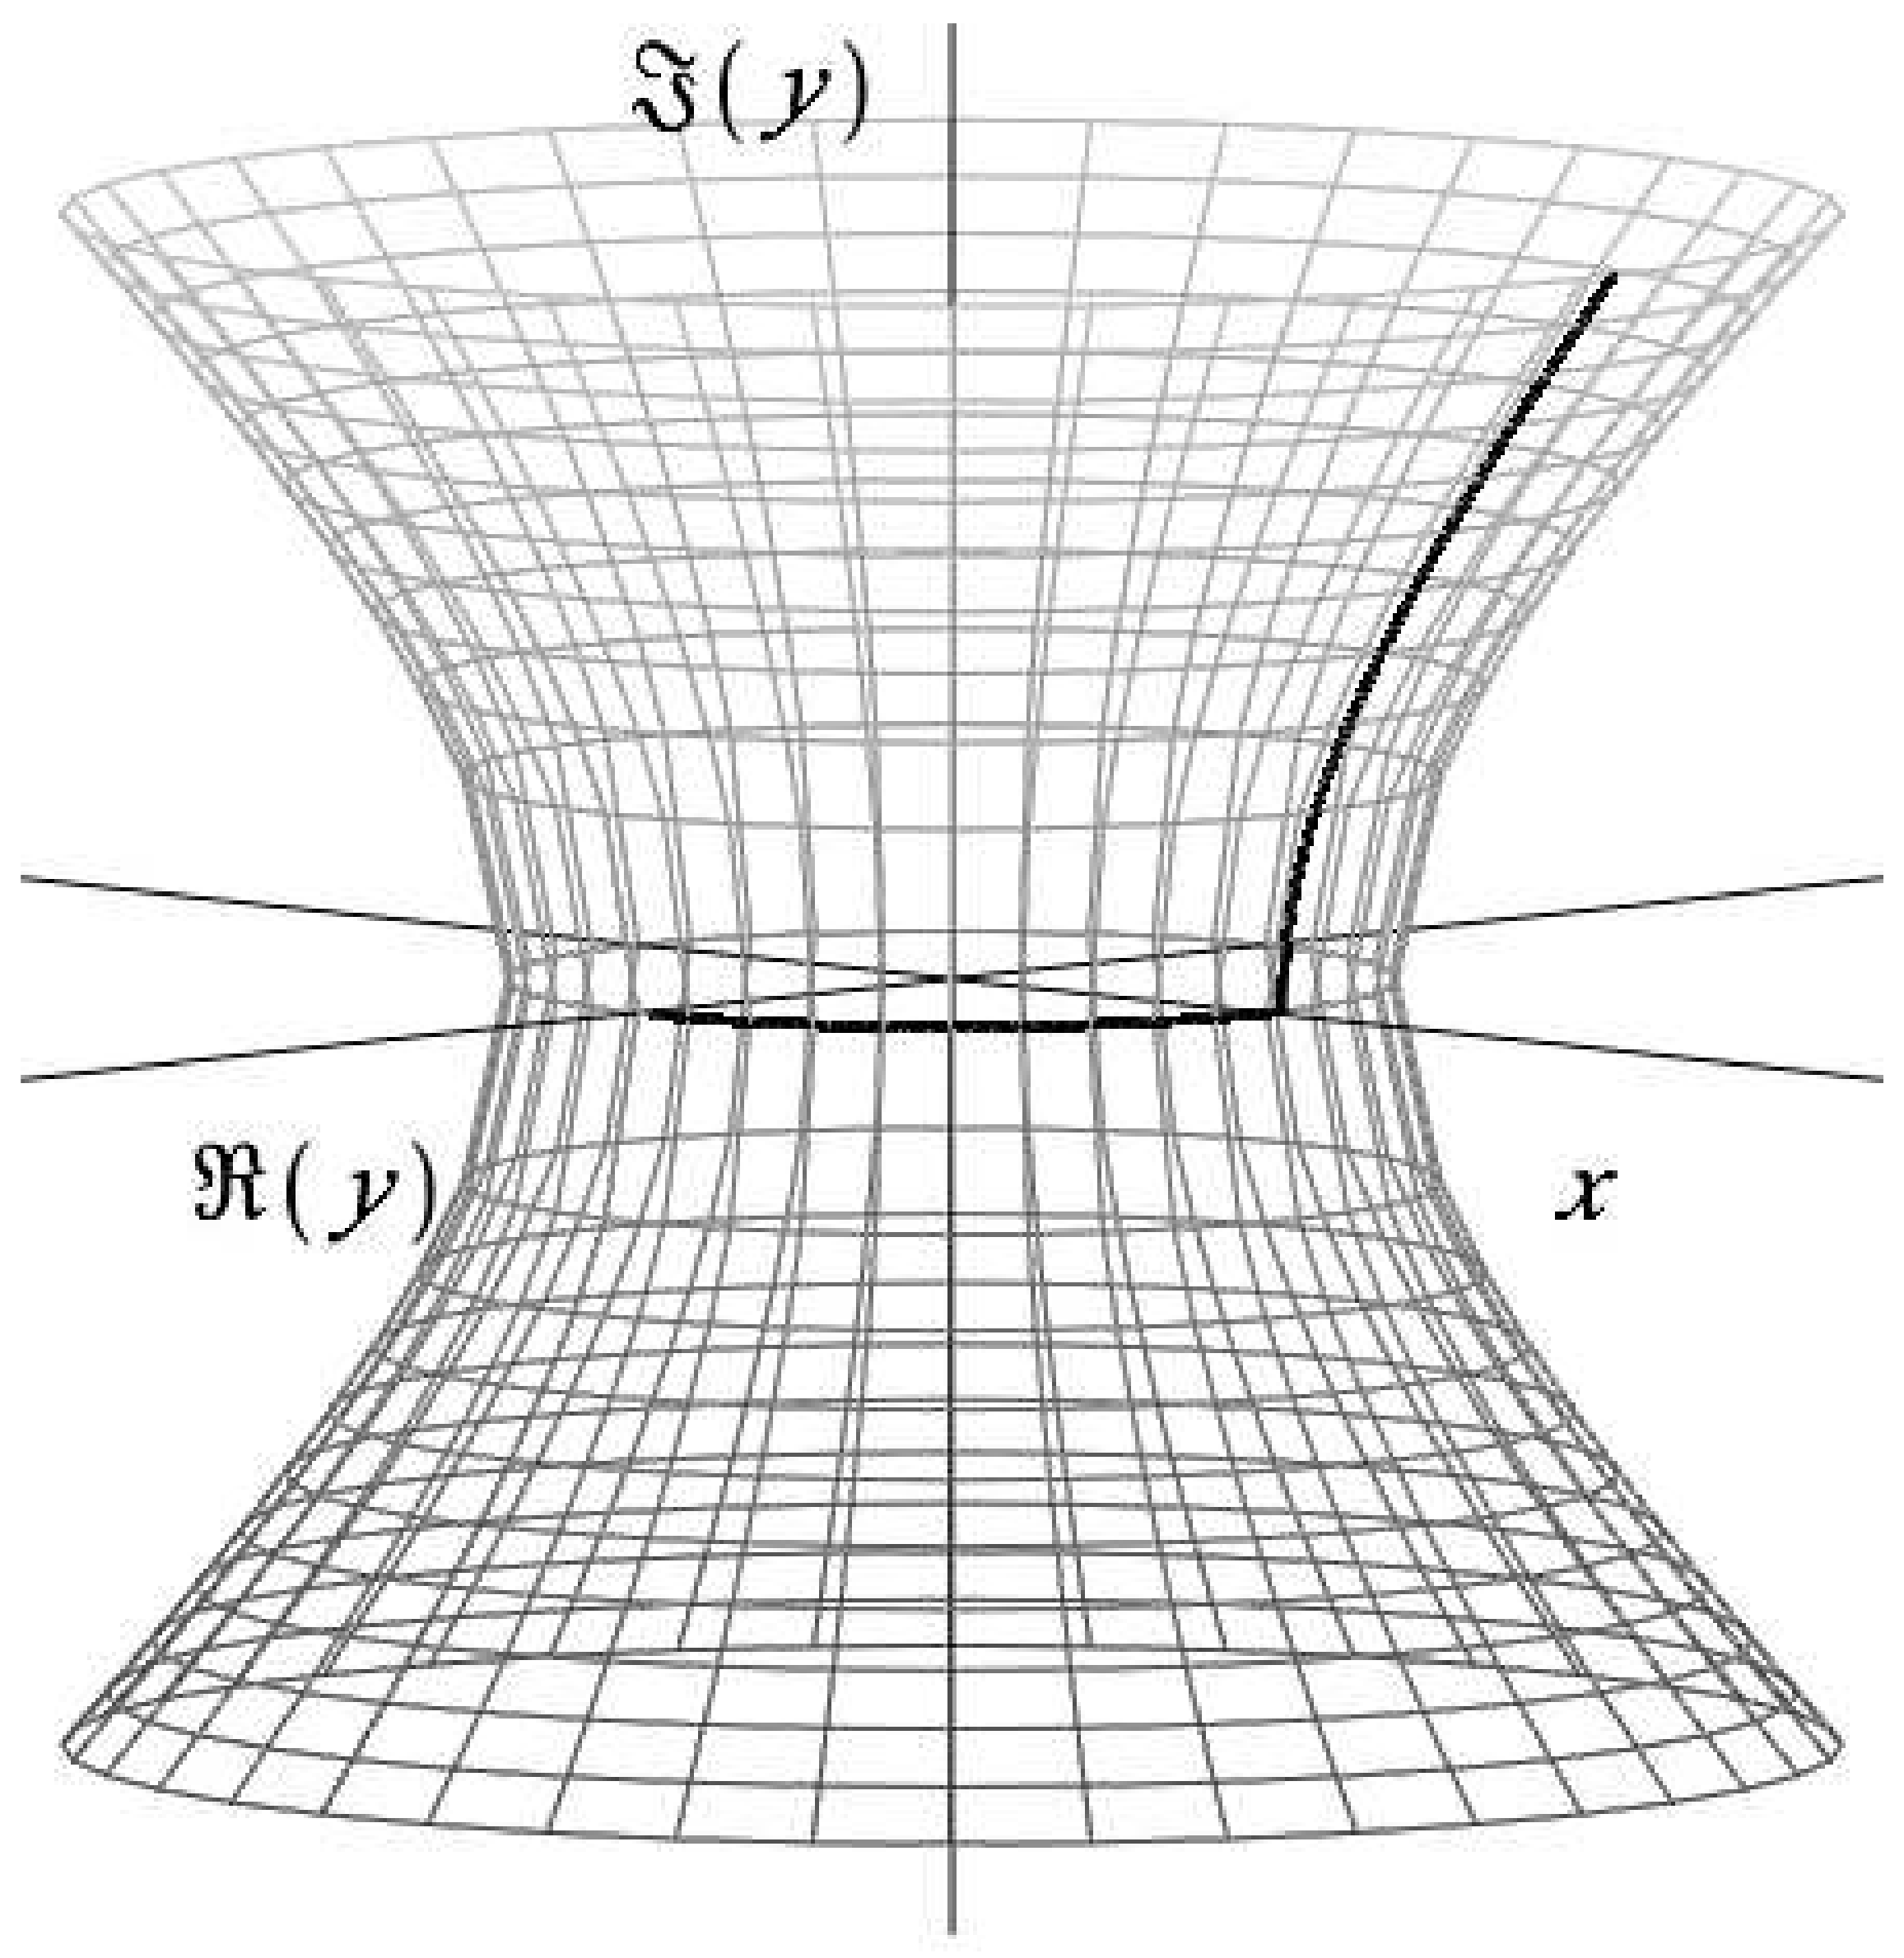
\includegraphics[height=2.9in]{../resources/PhD_thesis/max_symm_space_graphed.png}
\caption{The maximally symmetric surface as one continuous real manifold:
a spherical (Riemannian) cap joined at the equatorial throat to the
Lorentzian de~Sitter horn. The ninety-degree pivot at $r=\alpha$ is a
coordinate event on a single real surface, not a boundary of it. (2012
dissertation, \S sec\_RPT.)}\label{fig:maxsymm}
\end{figure}

% =====================================================================
\section{The $\Lambda$-completed vacuum as the universal standard of
physics}\label{sec:standard}
% =====================================================================

The real manifold of \S\ref{sec:real} is not an inert stage. Its curvature
radius $\alpha=\sqrt{3/\Lambda}$ is the one length the vacuum carries
intrinsically, and it is against that length---and against the null cone
locked to it (\S\ref{sec:rulings})---that everything else is measured. This
is the physical content of the cosmological constant, and it is why the
substrate is the object it is. The argument is Eddington's, sharpened by
the century since and by this corpus's results.

\subsection{Eddington's intuition, at weight}

Eddington read Einstein's law $R_{\mu\nu}=\Lambda g_{\mu\nu}$ as the
statement that the radius of curvature of empty space is a constant length
$\sqrt{3/\Lambda}$ in every direction at every
point~\cite{Eddington1923}. He then made the move that matters: length is
not absolute, so ``constant length'' can only mean constant \emph{relative
to the material standards of measurement}. Inverted, the law reads
\begin{quote}
\emph{The length of a specified material structure bears a constant ratio
to the radius of curvature of the world at the place and in the direction
in which it lies.}
\end{quote}
So the electron's radius in any direction is a numerical constant times the
radius of curvature of spacetime in that direction, and---his phrase---%
``an electron could never decide how large it ought to be unless there
existed some length independent of itself for it to compare itself with.''
Hence $\Lambda\neq0$ is not optional: without a finite intrinsic radius of
curvature there is no standard against which a material structure could be
what it is. The same reasoning takes the light cone $ds=0$ as the standard
of symmetry: ``symmetry itself can only be relative,'' and the propagation
of light is the standard it is relative to. \textbf{[established as
Eddington's argument, \cite{Eddington1923}; read here at weight.]}

This is the intuition Eddington packed into ``to drop the cosmical constant
would knock the bottom out of space''~\cite{Eddington1933}---a remark a
later generation dismissed~\cite{Chandrasekhar1983}, and which
Proposition~\ref{prop:unique} vindicates precisely: setting $\Lambda\le0$
removes the one real maximally symmetric manifold whose Lorentzian
signature is intrinsic, and so knocks the relativistic metrical structure
out of the vacuum.

\subsection{Where the intuition was right, foggy, and wrong}

Eddington reached the right object and misread its status, in ways the
present construction lets us correct sharply.

\emph{Right, and now unified.} He had two standards---a length standard (the
radius of curvature) and a symmetry standard (the light cone)---and left
them side by side. The equilateral-pseudo-sphere result unifies them: for
the one-sheeted hyperboloid, maximal symmetry forces the equilateral
profile $a=b$, whose asymptote is locked at the null cone and whose waist is
the curvature radius, so $c$ (the null-ruling gauge) and $\Lambda$ (the
scale) are the asymptote and waist of a \emph{single} surface, meeting in
the rate $H=c\sqrt{\Lambda/3}$ (\S\ref{sec:rulings};
\cite{JanzenCRframework}). Eddington's length standard and light-cone standard
are one standard, because the substrate that carries them is one
maximally symmetric object.

\emph{Foggy, and now overturned.} Eddington concluded that ``the symmetry
and homogeneity expressed by Einstein's law is not a property of the
external world, but a property of the operation of measurement''---the
anisotropy of a skewed world would enter both the measured structure and
the measuring rod and cancel. That deflation is the one thing the corpus
directly overturns. By \S\ref{sec:real} the maximally symmetric substrate
is the \emph{real intrinsic ground state} of the vacuum
(\cite{JanzenThesis}, whose maximal-symmetry result is stated for the
four-dimensional background; the void's basic state a real maximally
symmetric manifold), not an artefact of comparison. The symmetry
is a property of the world; and it is \emph{because} it is a real property
of the world---one standard, the same at every point---that measurement is
universal. Eddington had the dependence backwards: universality of
measurement is the \emph{consequence} of a real symmetric substrate, not the
\emph{source} of an apparent one.

\emph{Wrong, and now corrected.} Eddington held that there is ``no radius of
curvature in a timelike direction'' (he was working in Euclidean
coordinates with $x_4$ imaginary time), and drew from it that an electron,
having no temporal standard to measure itself against, ``just goes on
existing indefinitely.'' The error is exactly the imaginary-time misreading
\S\ref{sec:imaginary} dissolves: de~Sitter's Lorentzian signature is
intrinsic (Prop.~\ref{prop:unique}), its time-dimension as real as its
space-dimensions, so there \emph{is} a radius of curvature in the timelike
direction. The vacuum is a consistent measuring stick throughout space
\emph{and} time~\cite{JanzenThesis}---and that intrinsic temporal standard
is the objective cosmic-time lapse the programme later measures directly
from the redshift isotropy~\cite{JanzenModernParallax}. The electron's persistence
is not the absence of a temporal standard; the temporal standard is there,
and it is the same maximal symmetry.

\subsection{The universality of physics is the maximal symmetry}

Collecting the corrections gives the physical statement the geometric core
carries. The $\Lambda$-completed vacuum equation
$R_{\mu\nu}=\Lambda g_{\mu\nu}$ furnishes, in its unique intrinsically
Lorentzian maximally symmetric solution, the complete universal standard:
the intrinsic length $\alpha$, the intrinsic null structure $c$, and---%
correcting Eddington---an intrinsic temporal extent as real as the spatial
one, one standard isotropic about every point. \emph{That a specified
material structure is the same structure everywhere}---an electron bound for
the Coma cluster remaining an electron~\cite{JanzenThesis}---\emph{is the
statement that there is one standard everywhere, which is the statement that
the substrate is maximally symmetric.} The universality of physics is not an
added postulate laid over the geometry; it is the maximal symmetry of the
substrate, read as the constancy of the standard. And its necessity is
Eddington's ``$\Lambda$ cannot be zero'' grounded: a world that exists and
evolves requires a real intrinsic standard throughout space and time, which
is the necessary-and-sufficient augmentation of general relativity the
programme proves and measures~\cite{JanzenModernParallax,JanzenCRframework}.
\textbf{[reach --- the identification of universality-of-physics with the
substrate's maximal symmetry is the physical face of the paper's thesis;
each ingredient (the intrinsic standard, its necessity, the measured
temporal half) is established as cited, the identification the reach.]}

\subsection{The horizon problem, properly stated}

The same result settles, in the language cosmology already has a name for, a
problem usually posed the wrong way round. The horizon problem is standardly
stated as: why is the cosmic microwave background uniform to a part in
$10^{5}$ across regions that, on the standard expansion history, were never
in causal contact? So posed, it demands a \emph{mechanism} to communicate a
common condition across a horizon, and inflation supplies one. But the deeper
form of the question is not about temperature: it is why the electrons and
photons at the last-scattering surface are the same electrons and photons,
obeying the same physics, as those on Earth---how a causally distant patch
\emph{knows how to be} what our patch is. That is precisely the question the
preceding subsection answered for an electron bound for the Coma cluster: a
specified material structure is the same structure everywhere because there
is one intrinsic standard everywhere, which is the statement that the
substrate is maximally symmetric.

On the geometric core there is nothing to communicate. The universal
standard---the curvature length $\alpha$, the null cone locked to it, the
real temporal extent---is an intrinsic property of the one maximally
symmetric substrate (Prop.~\ref{prop:unique}), present at every point by the
symmetry itself, not a condition that had to propagate from region to region
and could therefore fall foul of a horizon. The uniformity is not the residue
of an early causal contact; it is the maximal symmetry of the substrate, the
very fact that makes physics universal. CR thus does not \emph{solve} the
horizon problem by finding a faster channel; it \emph{dissolves} it, by
locating the uniformity in the intrinsic standard rather than in a shared
past---there was never a gap to bridge. \textbf{[reach---the reading of the
CMB uniformity as an instance of the substrate's maximal symmetry, at the same
altitude as the universality-of-physics identification above; the intrinsic
standard is established (Prop.~\ref{prop:unique}), the identification the
reach.]}

% =====================================================================
\section{Reached through the imaginary, real everywhere it lands}\label{sec:imaginary}
% =====================================================================

Proposition~\ref{prop:unique} recasts every imaginary variable in the
construction as an instrument, not an ontological ingredient. Three
instances, each already in the corpus, are the same move:

\paragraph{The embedding coordinate.} $x_0\mapsto ix_0$ makes the surface
easy to see as a hyperboloid in $\mathbb{M}^5$; by
\S\ref{sec:real} it adds nothing to the manifold, which is the real
$(\mathbf{x})$ surface either way. The Riemannian and Lorentzian members
differ by their \emph{extrinsic} embedding curvature (Fig.~\ref{fig:sphere});
intrinsically each is a real manifold whose signature \eqref{eq:eigen}
reads off its own real metric.

\paragraph{The equatorial seam.} Where the slicing curve runs tangent to
the throat, the Riemannian cap joins the Lorentzian horn by the analytic
continuation $\theta\mapsto\pi/2+i\psi$, $\sin\theta\mapsto\cosh\psi$; the
signature of the \emph{two-dimensional slicing surface} flips because
$d\theta=i\,d\psi$ squares the continuation factor to
$-1$~\cite[prop.~flip]{JanzenSlicing}. The guard the slicing paper states,
and that this paper generalises, is decisive: \emph{the spacetime is
Lorentzian throughout}; the flip is confined to the $2$-surface, and the
continuation is a real analytic continuation ($\sin$ and $\cosh$ one
function), not a Wick rotation into a Euclidean spacetime. The seam is a
real feature of the real manifold, reached through an imaginary angle.

\paragraph{The cosmogenesis reassignment.} The correspondence that makes
collapsed matter a universe is a signature-\emph{preserving} causal
reassignment on the real Lorentzian horn; the compact Wick face, where a
continuous $\mathfrak{su}(3)$ would live, is real by construction but is
not a co-equal existent (it carries no clock)~\cite[\S
decoupling, \S face-status]{JanzenBoundary}. The matter rides the real
horn; the imaginary face is a face, not a second reality.

\begin{figure}[t]
\centering
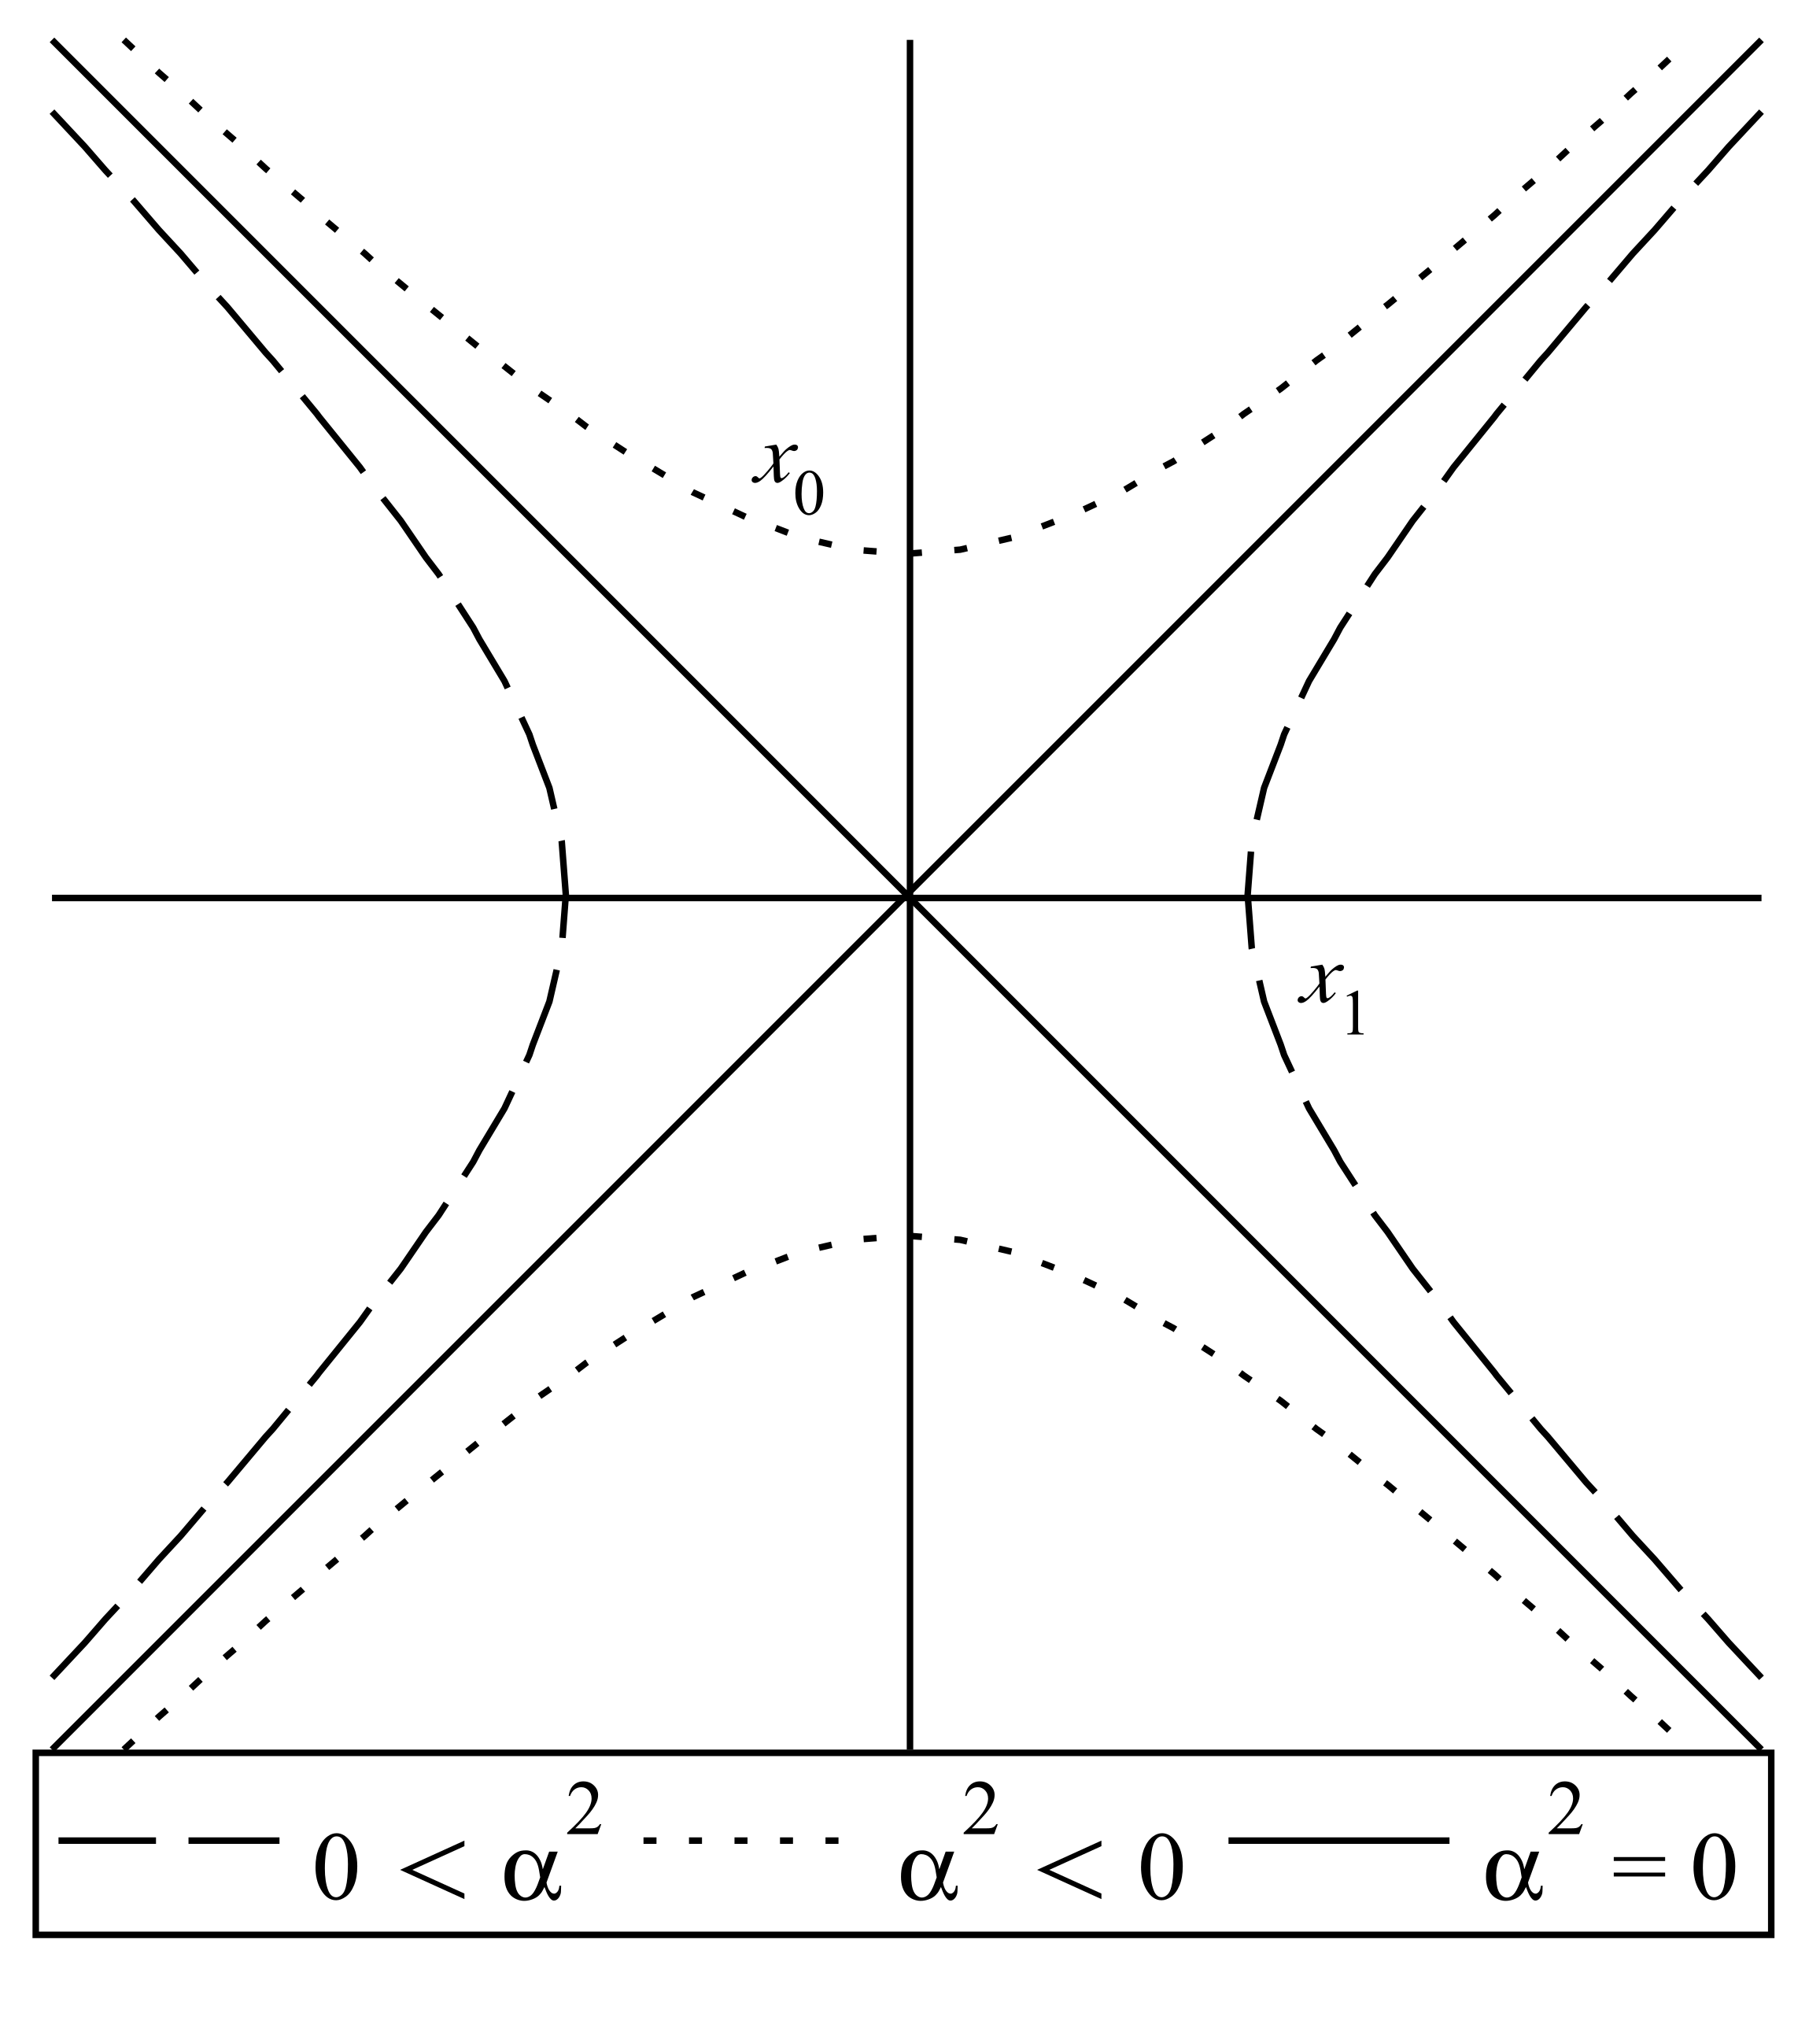
\includegraphics[width=3.0in]{../resources/PhD_thesis/Lorentz_sphere.png}\hfill
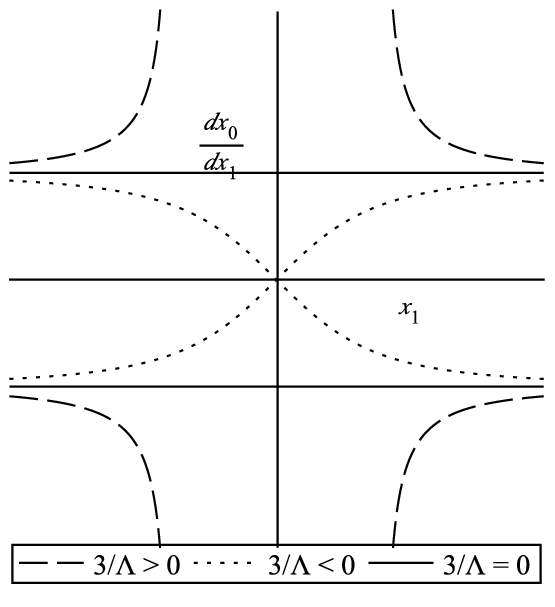
\includegraphics[width=3.0in]{../resources/PhD_thesis/Lorentz_sphere_diff.png}
\caption{The $\alpha^2$ family as spherical hypersurfaces of the embedding
space (left) and their differential character (right): de~Sitter
($\alpha^2>0$), anti-de~Sitter ($\alpha^2<0$), and the null cone
($\alpha^2=0$). The members differ by extrinsic embedding; each is
intrinsically a real four-manifold by \eqref{eq:sphere3}. (2012
dissertation.)}\label{fig:sphere}
\end{figure}

\begin{remark}[the general statement]
Each bullet is a place the corpus already refuses the unreal reading. The
paper's contribution is to state the \emph{general} law they instance: the
construction reaches a real manifold through imaginary instruments, and the
geometry is intrinsically real at every point they land on---substrate,
seam, cosmogenesis, and the phase structure hypothesised at the seam
relative to trajectories. This is CR's \emph{built-by-construction-and-real}
register; reading the imaginary parametrisation as rendering anything
\emph{unreal} is the invented flaw the discipline is built to
defeat~\cite{JanzenShadowExistence}. \textbf{[established for the substrate, the seam
as a geometric object, and the cosmogenesis reassignment (sources above);
the phase-structure-at-the-seam reading relative to trajectories is a
\textnormal{[reach]} held do-not-assert --- the interpretive layer the
conjugacy programme opens, geometric base real, trajectory/phase reading
open.]}
\end{remark}

% =====================================================================
\section{The straight null rulings: the light cone is the visible peak}\label{sec:rulings}
% =====================================================================

The most visible face of the intrinsically real geometry is its null
structure, and it was drawn in the same dissertation chapter. On de~Sitter
the null condition $0=-dx_0^2+\sum_i dx_i^2$ makes the null-lines
\emph{straight lines} on the curved real surface in the flat embedding: a
null particle traverses an angle $\pi/2$ on $\alpha<r<\infty$, and two
null-lines separated by $\pi$ at the throat run parallel through the
embedding and never meet~\cite[Eqs.~following (null\_eom)]{JanzenThesis}.
The surface is \emph{doubly ruled by straight null lines}, and the rulings
are the reassigned generators the null-boundary correspondence acts
on~\cite{JanzenCRcosmology}.

This is the geometric substrate of the $c$--$\Lambda$ result the framework
paper now carries~\cite[\S 662-region]{JanzenCRframework}: for a one-sheeted
hyperboloid, maximal symmetry forces the \emph{equilateral} member
$a=b$---the profile whose rulings meet perpendicular at the throat and
whose asymptote is locked at the null cone---so $c$ is the null-ruling
gauge, $\Lambda$ the sole free scale, and the two meet only in the
expansion rate $H=c\sqrt{\Lambda/3}$, with the curvature--tilt relation
$\tan\theta=a\sqrt{-K}$ specialising to the locked cone. What
\S\ref{sec:real} adds is the ontological reading of this: the rulings are
\emph{real straight lines on a real surface}; $c$ fixes their slope, the
throat curvature $1/\alpha^2$ their scale, and both are intrinsic to the
one real equilateral pseudo-sphere. The $c$--$\Lambda$ structure of the
framework paper is the tip; the intrinsically real ruled geometry is the
iceberg beneath it. \textbf{[established --- the rulings
\cite{JanzenThesis}; the equilateral-forcing and $c$--$\Lambda$
\cite{JanzenCRframework}; the ontological reading collected here.]}

\subsection{The power of a point is the height: the null structure in Euclid's own quantity}\label{sec:power}

The rulings are the substrate's null structure seen from outside. There is a
second face of the same fact, and it is older than the geometry: the null
condition on this surface \emph{is} a classical theorem about circles, and the
theorem is about the throat.

Read the substrate's overhead projection---the equatorial plane, on which the
throat is a circle of radius $\alpha$. For a point $P$ of the projection at
distance $|X|$ from the axis, the \emph{power} of $P$ with respect to that
circle is
\begin{equation}\label{eq:power}
\mathrm{pow}(P)\;=\;|X|^{2}-\alpha^{2},
\end{equation}
the invariant Steiner attached to a point in 1826~\cite{Steiner1826}: the
constant value of $\overline{PA}\cdot\overline{PB}$ along every line through
$P$ meeting the circle at $A,B$, and, for $P$ outside, the square of the tangent
length (Euclid III.36~\cite{Euclid}). But the hyperboloid
$-x_{0}^{2}+|X|^{2}=\alpha^{2}$ says that the same combination is the point's
own height,
\begin{equation}\label{eq:powerisheight}
|X|^{2}-\alpha^{2}\;=\;x_{0}^{2}.
\end{equation}
So $\mathrm{pow}(P)=x_{0}^{2}$: \emph{the power of a point with respect to the
throat is the square of its height in the embedding.} The tangent from $P$ has
length $\sqrt{\mathrm{pow}(P)}=|x_{0}|$; it therefore runs exactly as far across
as the point stands high, and in a metric of signature $(-,+,\dots,+)$ that is
$\mathrm{d}s^{2}=-x_{0}^{2}+|x_{0}|^{2}=0$.

\begin{proposition}[The tangent is a null line]\label{prop:tangentnull}
The tangent line from any point of the substrate to the throat is a null line of
the embedding. Equivalently: Euclid's tangent--secant relation and the null
condition are the same equation, and the only thing that turns one into the
other is the minus sign in the metric.
\end{proposition}

\begin{proof}
$\mathrm{tangent}^{2}=|X|^{2}-\alpha^{2}$ is Euclid III.36 read through
Pythagoras on the radius--tangent right angle; $x_{0}^{2}=|X|^{2}-\alpha^{2}$ is
\eqref{eq:powerisheight}. Hence (spatial run)$^{2}=$ (time drop)$^{2}$ and
$\mathrm{d}s^{2}=0$. (Verified numerically at the hinge and at $600$ random
heights, $\max|\mathrm{d}s^{2}|=5.7\times10^{-14}$; receipts:
\texttt{power\_of\_a\_point.py}\rcpt{P17_power_of_a_point}, \texttt{power\_is\_null.py}\rcpt{P17_power_is_null}.)
\end{proof}

This is the rulings of \S\ref{sec:rulings} in a second register, and the two
identify: a ruling meets the throat tangentially, so the rulings \emph{are} the
tangents Proposition~\ref{prop:tangentnull} describes, and ``doubly ruled by
straight null lines'' and ``every tangent to the throat is null'' are one
statement. What the classical register adds is reach: the proposition is about
\emph{every} point of the overhead, not only the ones a ruling happens to pass
through. The sightlines of the projection that \emph{touch} the throat are light
rays; those that \emph{cut} it are not, and the distinction is Euclid's own---the
power theorem is about secants, and the null condition is its degenerate case,
where the secant's two points merge. The null character is the embedding's, and
it is worth being exact about where it lives: the equatorial plane carries a
positive-definite restriction of $\eta$, so no displacement \emph{within} the
plane is null. What is null is the corresponding displacement on the substrate,
from the vantage lifted to its own height $X_{0}=\sqrt{\mathrm{pow}}$ to the
point of tangency\rcpt{O2_sightline_null_on_lift}. The planar figure is the
shadow of that null line, which is why the power of a point reads the light cone
at all. \emph{The tangent is exactly where the
light cone is.}

\begin{remark}[One privileged circle]\label{rem:onecircle}
The identity $\mathrm{pow}=x_{0}^{2}$ is not a fact about powers. It is a fact
about \emph{one} circle: the substrate's waist. A power taken with respect to any
other circle of the projection is a perfectly good Euclidean quantity and is not
a height, because \eqref{eq:powerisheight} is the hyperboloid's equation and the
hyperboloid has one waist. This bounds sharply what classical circle geometry can
say here: a theorem whose quantity is built from the power with respect to the
throat carries the signature for free; a theorem whose quantity is a chord
(Ptolemy~\cite{CoxeterGreitzer1967}), a bilinear relation among points (La
Hire's reciprocity~\cite{Coxeter1987b}), or a power with respect to some other
circle (Casey's bitangents~\cite{Casey1866}) carries no height at all
and returns Euclid unchanged. The boundary is not a defect of the reading. It is
the statement that the substrate has exactly one waist, met in the classical
language. The bound is not an artefact of working in the projection either. And the polarity has a second thing to say about the figure, which is what a projective reading is for: it dualises it. Duality with respect to the throat carries points to lines and reverses incidence, so the pencil of slicing planes through a hinge goes over to the range of points on that hinge's polar. That polar is computed in one line---the hinge sits at transverse $2\alpha$, so its polar is the line at $\alpha/2$---and it is not a new line in the figure: it is \emph{the opposite side of the contact triangle}, whose vertices are the three points at which the hinge triangle's sides touch the throat, the midpoints of the companion slicing paper's midpoint-tangency statement~\cite{JanzenSlicing}%  r2376+c54.9: was \ref{prop:twoalpha}, a label that lives in P3 -- \ref does not cross papers, so it printed as ??
\rcpt{D1_hinge_duality}. The dual of the hinge triangle is therefore the contact triangle, the dual of the swing is a point sliding along one of its sides, and the throat is self-dual, being the conic of the duality. The self-conjugate case is the throat-tangent door, whose pole is its own point of contact. \emph{The corpus had the dual figure drawn from the beginning}---the tangency points are the same three the hinge placement already turns on---and read it only as a set of midpoints. The
polarity of the embedding quadric itself---$P\mapsto\{X:\eta(P,X)=\alpha^{2}\}$,
which depends on the single invariant $\eta(P,P)$ against $\alpha^{2}$---returns
at each named point exactly what \eqref{eq:powerisheight} already gives, since
that identity is the hyperboloid's equation. One further projective question closes here rather than opening, and the closure is worth stating because it is the one-scale result met from a new side. The classification of a \emph{pencil} of quadrics by its elementary divisors asks how two quadrics sit relative to one another; applied to this figure it returns nothing, and cannot. Every conic the construction owns is manufactured from the throat---the throat itself at $\alpha$, the hinge circumcircle at $2\alpha$ which \S\ref{sec:rulings} derives as the circle on the throat's own edge through its own centre, the contact triangle's circumcircle which is the throat again, and that triangle's incircle at $\alpha/2$. Taking the throat with the hinge circumcircle and computing the pencil's degeneracies returns the doubled line at infinity, which is precisely the classical signature of concentricity\rcpt{D3_segre_no_pencil}: the classification hands back the manufacture. \emph{A second quadric in general position would be a second scale, and the construction has one}---so the absence of a Segre problem here is the one-scale result read from the pencil side, and not a gap in the reading. The hinges are the case in point:
each lies \emph{on} the quadric ($-3\alpha^{2}+4\alpha^{2}=\alpha^{2}$), so its
polar is the tangent hyperplane there, and the tangent length $\sqrt3\,\alpha$
from the foot of its axis is \eqref{eq:powerisheight} evaluated at transverse
radius $2\alpha$ rather than an independent
relation.\rcpt{Q1_quadric_polarity}
\end{remark}

Two ingredients of \eqref{eq:powerisheight} are modern and it is worth marking
both, since the temptation is to count one. The first is the minus sign---the
Lorentzian signature, without which the tangent's length and the point's height
are two numbers that happen to agree. The second is \emph{power itself}: Euclid
proves a relation among segments; it was Steiner who shifted the focus from the
chords to the point and named $|d^{2}-r^{2}|$ an invariant belonging to
it~\cite{Steiner1826}. Equation~\eqref{eq:powerisheight} needs the invariant, not
the relation. That second move is the one this programme makes everywhere: it is
the same move as reading the cut's offset $r_{0}$ not as a coordinate of the
construction but as the mass itself~\cite{JanzenSlicing,JanzenOperator}.
\textbf{[established --- \eqref{eq:power}--\eqref{eq:powerisheight} and
Proposition~\ref{prop:tangentnull} are identities, verified; the
one-circle bound of Remark~\ref{rem:onecircle} is established by the
identity's own dependence on the waist; the historiographic reading is
collected here.]} The bound of Remark~\ref{rem:onecircle}
is not a conjecture about what classical geometry might fail to say: it was found
by running the classical catalogue against the throat one theorem at a time, and
the boundary is where the run stopped paying. The pole--polar relation, the radical
axis of the throat and the circle that places the hinge, and inversion in the throat
each return the same object---the chord of contact of a point's two null tangents,
which is that point's horizon on the throat---by three routes sharing no machinery;
Ptolemy, La~Hire's reciprocity, and Casey's bitangent identity~\cite{CoxeterGreitzer1967,Coxeter1987b,Casey1866} each hold on the
figure and return nothing, for the three reasons the remark names. The catalogue,
its receipts, and the failures that drew the boundary are recorded in the
programme's figure-theorem ledger (\texttt{FIGURE\_THEOREM\_LEDGER.md}, with
\texttt{storyboard\_receipts/}); what is carried here is the identity, its bound, and what the run returned.

Two things about that boundary are worth stating together, because they are the
reason to trust the reading rather than merely to admire it. The first is that it
was \emph{found}, not posited: the classical catalogue was run against the throat
one theorem at a time, and the boundary is where the run stopped paying. The
second is what the run returned when it did pay. The pole--polar relation gives
the chord of contact of a point's two null tangents; the radical axis of the
throat and the circle that places the hinge gives the same line without mentioning
a tangent; inversion in the throat gives it a third time, as the image of that
circle. Three classical constructions sharing no machinery, one line---and the
line is the vantage's horizon. None of the three is confined to the equatorial
figure. The pole--polar relation is the quadric's own, and returns there what
\eqref{eq:powerisheight} already gives\rcpt{Q1_quadric_polarity}; inversion in
the throat extends as the algebraic identity $\eta(P,P^{*})=\alpha^{2}$ for
$P^{*}=\alpha^{2}P/\eta(P,P)$, holding off the equatorial plane and at either
signature of $\eta(P,P)$, an involution whose fixed set is the whole substrate
of which the throat is the equatorial section\rcpt{C3_inversion_extends}. The
bound of Remark~\ref{rem:onecircle} therefore governs all three routes in the
full space exactly as it governs them in the projection. Euclid's tangent--secant theorem, read on the same
figure, locates the light cone: along a sightline through the throat the near
intersection is timelike-separated from the vantage and the far one spacelike, and
the interval vanishes at the geometric mean of the two segments---exactly the
quantity III.36 identifies as the tangent length. The triple-angle identity returns
the Nariai configuration. The nine-point circle of the hinge triangle \emph{is} the
throat.

\emph{None of that is new physics, and that is the point.} Every one of those
results is already established in this corpus---the horizon, the light cone,
Nariai, the throat's radius, the perspectival reading of the mass---and each is
reached here by a route sharing no machinery with the one that established it. A
reading that returned new physics from a two-thousand-year-old theorem about
circles would be an object of suspicion; one that returns what the construction
already proved, repeatedly and from unrelated directions, is doing what a faithful
dictionary does. The classical geometry is therefore not evidence for the physics,
and is not offered as any: it is a second way of seeing an object the construction
arrived at first, and the agreement of the two readings is the only thing either
can honestly be cited for. Nor is the reach of the agreement a mystery to be
marvelled at. That so much of the classical theory of the circle turns out to speak
about causal structure is accounted for entirely by
Remark~\ref{rem:onecircle}: it speaks about causal structure exactly when it speaks
about the power of a point with respect to this one circle, and this one circle is
the waist of the substrate.

% =====================================================================
\section{Maximal symmetry, worn seven ways}\label{sec:unification}
% =====================================================================

The reality of the substrate is the reality of \emph{the} maximally
symmetric Lorentzian manifold (Prop.~\ref{prop:unique}); its standard-hood
is that same manifold serving as the universal measure (\S\ref{sec:standard}).
We now state the third face: that maximal symmetry---the isometry group
$SO(5,1)$ complete and exhausted---is the single root of seven results the
corpus establishes separately. And the list has a geometric substrate of its own worth naming before it is read: the four-geometries it ranges over are the polar slices of the substrate's own points (\S\ref{sec:rulings}), one background for each point and none privileged, so \emph{the many ways the substrate is read are indexed by the substrate itself}\rcpt{Q6r_polar_is_the_background}. \textbf{[reach --- the seven are each
established; reading them as one fact is the thesis, decidable by the test
in \S\ref{sec:frontiers}.]}

\begin{enumerate}
\item \textbf{Necessity and sufficiency of the augmentation.} CR is the
necessary and sufficient augmentation of general relativity for a
description of structural existence, the necessary half
measured~\cite{JanzenModernParallax,JanzenCRframework}. Maximal symmetry is what
makes the substrate the least-arbitrary vacuum such a description can be cut
from---least-arbitrariness being the programme's own criterion of necessity
(Rule~2 of~\cite{JanzenShadowExistence}, read in the ontological register): a
symmetry-breaking modulus is the adjustable parameter that criterion rejects,
and maximal symmetry the unique structure that requires its configuration, so
the substrate's selection is an instance of the discipline's own load-bearing
rule rather than an added axiom.
\item \textbf{The constraint algebra is the symmetric-space grading.}
General relativity's own hypersurface-deformation (Dirac) algebra \emph{is}
the symmetric-space grading $\mathfrak{so}(5,1)=\mathfrak{h}\oplus\mathfrak{m}$ of the substrate---two
normal deformations bracketing into a tangential one being exactly two coset
directions bracketing into the isotropy, term for term---and the
``wrong-sign'' structure function standardly recognized at the root of the
problem of time \emph{is} the substrate's own Lorentzian coset metric, so the
obstruction dissolves into a single geometric fact: the base-dependence of
that metric~\cite{JanzenAlgebroid}. Maximal symmetry, read at the canonical
rung, is what GR's constraint algebra already \emph{was} and what dissolves
its problem of time---established on the symmetry-reducible sector, the
finite $\mathfrak{so}(5,1)$ reduction.
\item \textbf{One scale; the constants are gauges.} The substrate carries a
single dimensionful scale, $\Lambda$; the constants through which physics is
written on it are unit gauges. $c$ is the null-ruling slope of the equilateral
pseudo-sphere (\S\ref{sec:rulings}), meeting $\Lambda$ dimensionally only in
$H=c\sqrt{\Lambda/3}$; $G$ never appears alone but only as the source's
gravitational radius $GM/c^2$, the mass $M$ perspectival and fixed to the
Nariai value by $\Lambda$ in the cosmology ($\Lambda G^2M^2/c^4=1/9$)~\cite{JanzenCRframework};
$\hbar$ enters only at the seam, scaled by $\Lambda$ alone, the de~Sitter
horizon's thermal state~\cite{GibbonsHawking1977} closing the scale factor's lone self-adjoint-extension
freedom \emph{without a free parameter}~\cite{JanzenCanonicalTime}; and $k_B$
converts that horizon temperature to energy. So the
gravitational--cosmological--quantum sector spends \emph{no free dimensionless
constant}---every would-be free parameter is a unit gauge or a freedom maximal
symmetry has already spent (the perspectival mass fixed at Nariai, the
quantization closed by the horizon). \textbf{[reach --- the source facts are
each established and cited; reading the sector's free-data count as zero, so
that the theory's free data is carried entirely by the matter, is the thesis,
decidable by the count in \S\ref{sec:frontiers}.]}
\item \textbf{The cosmology is parameter-free.} With $\Lambda$ the sole
scale, the low-multipole deficit, the transmission character, and the
radiation-free expansion rate carry no tunable freedom---the rigidity whose
two-sidedness (match on the rate and the abundances; a parameter-free,
falsifiable prediction on the acoustic shape---the low-multipole a
cosmic-variance-limited wash, the damping scale a genuine open build) is the
discriminating power, the one measured initial condition $\rho_r/\rho_m$ an
$\eta$-analogue \emph{read} not tuned~\cite{JanzenCRcosmology}.
\item \textbf{The continuous matter symmetry is walled.}
$\mathfrak{su}(3)\not\subset\mathfrak{so}(5,1)$ precisely because $SO(5,1)$
is exhausted; the same completeness that locks the constants leaves no room
in the continuous isometry for a geometric colour~\cite{JanzenBoundary}.
The complement is not empty, and the same completeness fixes it: the
substrate $\mathrm{dS}_5=SO(5,1)/SO(4,1)$ is topologically $\mathbb{R}\times
S^4$, hence spin with a \emph{unique} spin structure, inherited by the
four-dimensional cut; and the one orientation parity
$R\in\mathrm{O}(5,1)\setminus\mathrm{SO}_0$~\cite{JanzenAlgebroid} reflects the
cut-normal ($r_0$) direction, acting on the cut's natural spinor as the chirality operator $\gamma^5$
itself---the cut-normal being the transverse mass-modulus (the offset $r_0$
that \emph{is} the mass), whose $\mathrm{Cl}(1,4)$ generator is $\gamma^5$---so
the substrate's single orientation $\mathbb{Z}_2$ \emph{is} the chirality
grading, measuring left against right as it carries the graviton's helicities. \emph{And the discrete residue is larger than the orientation parity alone, by a route that uses only what
the substrate already carries.} The horizon roots carry surface gravities, hence a residue pairing on the
triple; that pairing has a holonomy about the branch points---the per-root resolution of a square root the
Galois statement takes in the product---and adjoined to the deck symmetry it closes the Weyl group of
$\so(6,\mathbb{C})$, this substrate's own complexified isometry
algebra~\cite{JanzenGroupoid, JanzenAlgebroid}. \emph{The $A_2$ the corpus reads off the cubic is the
sub-root-system obtained by deleting one node of that $A_3$}, so the discrete structure is not an addition to
the object but a fuller reading of it---which is this paper's thesis applied to itself.
So the exhausted isometry does not merely wall a continuous matter symmetry; it
fixes a discrete one, the fermion chirality identified with the substrate's own
orientation parity. What the residue supplies is the fermion sector's arena, its chirality grading, and its discrete generation-structure---built and forced within CR, no longer the conjecture this line carried before r1609; the content it grades---the mass values, the electroweak scale---is the ordinary route, not the geometry's, so CR's claim is a gravitational--cosmological unification, not a geometric unification of matter~\cite{JanzenBoundary}. The residue's discrete content is moreover a linear orientation skeleton---the parity $P$, a time reflection $T$, the $\gamma^5$ grading, and the $R$-parity carrying the fundamental $\mathbf 3$ to its antifundamental $\bar{\mathbf 3}$---whereas charge conjugation, antilinear where those act linearly, is field-level like the charge it acts on (the substrate carrying it as a symmetry and not a datum---the metric even in the charge, its sign the bend of the cut~\cite{JanzenRange}); so a geometric $CPT$ is not auto-yielded, the geometry supplying the orientation \emph{skeleton} of matter \emph{and its antimatter}---the discrete $\mathbf 3\oplus\bar{\mathbf 3}$ the $R$-parity relates, matter and antimatter at one weight within CR~\cite{JanzenMatter}---and not the charge, which is field-level on both branches alike---the same partition once more, the residue the arena, the grading, and the skeleton, the content and the charge the ordinary route~\cite{JanzenBoundary}. The antilinear structure is not, however, exhausted by the field level, and the boundary the residue draws encloses a positive shape: the reality involution $\tilde\tau\mapsto\bar{\tilde\tau}$ on complexified cosmic time is antilinear \emph{and} geometric, so charge conjugation factorises into a geometric kinematic (Feynman--St\"uckelberg) face---carried by the bead's own $r=0$ crossing, so that the cosmogenesis carries $C$'s kinematic content---and the field-level charge sign alone, a geometric $CPT$ staying unyielded because only the charge closes from the field, and this face realised on the built fermion sector's zero-modes~\cite{JanzenBoundary,JanzenMatter}.
\textbf{[reach --- the spin structure and the $\gamma^5$-action are grounded:
the parity \emph{measures} chirality (the exchange reading excluded by explicit
computation, since $R$ reflects the transverse cut-normal and fixes the four
spacetime legs), detailed in the boundary paper~\cite{JanzenBoundary}; the
same parity grades mass in \emph{both} faces---the geometric mass-reflection
$r_0\mapsto-r_0$ (whence $2M\mapsto-2M$) and the $R$-odd fermion mass term---so
mass, geometric or fermionic, is the substrate's one $R$-odd datum.
\emph{And that identification carries further than it has been read, so we develop it here rather than leave it
in a clause.} Read at the electroweak sector it says that what the \emph{Higgs mechanism} breaks is this
parity: the $R$-symmetric sector is the offset-free, massless configuration and mass is the $R$-odd departure
from it. \emph{What is thereby claimed is a mechanism and not a magnitude}---the vacuum expectation value, the
electroweak scale and the individual masses stay the ordinary route, as this paper says throughout and as the
one-constant structure requires. \emph{But three things follow that were not being said, and each is a
property of the slicing relation the companion paper already
carries}\rcpt{P0_the_order_parameter_is_the_offset_and_it_is_bounded_by_the_nariai_member}, $2M=r_{0}-r_{0}^{3}$ in the gauge $\alpha=1$~\cite{JanzenSlicing}.
\emph{First, the mass-reflection above is an identity of that relation rather than a further assumption}: the
cubic is odd, so $r_{0}\mapsto-r_{0}$ sends $2M\mapsto-2M$ exactly.
\emph{Second, the symmetric sector is the bare substrate.} $2M=0$ at $r_{0}=0,\pm\alpha$, and the metric
function is $1-r^{2}/\alpha^{2}$ at all three---one massless geometry read at three offsets, so the unbroken
phase of this breaking is de~Sitter itself and not a separate configuration.
\emph{Third, and this is the part that distinguishes the geometric statement from the field-theoretic one it
is being set beside: the order parameter is bounded, and its bound is the degenerate member.} Over the
admissible offsets $|r_{0}|\le2\alpha/\sqrt3$---the regime range the slicing paper reads off the discriminant
$4-3r_{0}^{2}$---the mass satisfies $|M|\le\alpha/3\sqrt3$, with equality at $r_{0}=\pm\alpha/\sqrt3$ and at
the range endpoints, and that value is the Nariai mass, obtained independently as the double root of the
horizon cubic. \emph{A quartic potential is unbounded in its field; this order parameter is not, and it
saturates exactly at the configuration a collapse reaches}~\cite{JanzenCRframework}.
\emph{And the breaking has a cause here rather than a chosen minimum.} The companion paper does not posit the
offset: it derives that a manifold observer cannot be assumed to sit at $r_{0}=0$, because the reference such
an observer actually has is the hole's image on their celestial sphere and there is no marked point on that
image for a reticle to land on~\cite{JanzenSlicing}. \emph{So on this reading the symmetry is broken because
of what a reference is, not because a potential was written with its minimum away from the origin.}
\emph{We state the limits of that with the same care.} No vacuum expectation value, no scale and no mass value
follows from any of it; nothing here derives the Higgs field, its potential, or the gauge group it breaks---and
if that group were ever promoted from described to forced, the relation this paper draws to it would have to be
re-examined rather than inherited~\cite{JanzenBoundary}. One
candidate centrepiece stands here, stated at what it has since become rather than at what it was when first written (r1609): the residue's
full automorphism $\mathrm{Aut}(A_2)=S_3\times\mathbb{Z}_2\cong D_6$, read on a
fermion sector, carries the shape $3\times2$---three generations times two
chiralities---the $\mathbb{Z}_2$ the $\gamma^5$ grading just fixed, the $S_3$
permuting the three mass-tied roots of the offset-mass cubic (the discrete
$\mathfrak{su}(3)$-Cartan--Weyl shadow~\cite{JanzenAlgebroid}), a $2M$-degenerate
flavour triplet whose hierarchy would be a separate breaking; the chirality
factor grounded, and the generation factor since \emph{built} and forced within
CR~\cite{JanzenMatter}; only the descent onto a \emph{propagating} spinor sector is still held
do-not-assert, and it is the corpus's open family~6 rather than an unrouted gap. The same $A_2$ skeleton is now realised in the geometry itself: the slicing paper draws the hexad as a skew hexagon of null rulings across the substrate's two horns, each horn's three vantage-hinges designating the three roots~\cite{JanzenSlicing}. Whether that geometric six-fold is the \emph{same} hexad as the flavour triplet here---the one exchanged by the geometric time reflection, the other by the offset parity $R$, two distinct $\mathrm{O}(5,1)$ reflections that both swap the null rulings---or a resonance of shared abstract type, is \emph{settled} rather than open: the slicing paper establishes it as a resonance and \emph{not} an identity---the horn-swap $T$ (timelike, horn-flipping) and the offset parity $R$ (spacelike, horn-preserving) being distinct reflections that share the fundamental triple and complete it distinctly~\cite{JanzenSlicing}, verified on the six points. The chiral content this parity would grade is
not built here.]}
\item \textbf{One circle: the equator is what the construction is built on.} The substrate has exactly one waist (Rem.~\ref{rem:onecircle}), and its radius \emph{is} the curvature: $\alpha=\sqrt{3/\Lambda}$, the sole scale (\S\ref{sec:standard}). What the construction is built from is a set of facts about that one circle, and they are one fact. The power of a point with respect to it is the square of the point's height, \eqref{eq:powerisheight}, so the tangent to it from any point of the substrate is null (Prop.~\ref{prop:tangentnull}) and the rulings \emph{are} those tangents (\S\ref{sec:rulings}): the double ruling and the classical power law are the same statement, set by $\alpha$ and by nothing else, and the power vanishes identically on the circle itself ($x_{0}=0$). That circle is the incircle of the hinge triangle and its nine-point circle besides, so the hinges stand at $2\alpha$ as an \emph{output} of the hole rather than a stipulation, the three sides are the Nariai double null rulings tangent at their midpoints, and the triple-angle identity returns the Nariai configuration of its own accord~\cite{JanzenSlicing}. The signed areal radius passes through zero at a point \emph{on} that circle, so the three hinges' walls lie on it as a $\mathbb{Z}_3$-orbit whose three-foldness is the hole's own, and the fermion sector's three chiral generations are those three walls~\cite{JanzenMatter}. The slicing's lap runs around it, and through it the cosmological gravitational collapse of a black hole in a prior universe completes into the formation of a universe like our own---collapsed matter cannot terminate but continues as a cosmology---matter and antimatter the two ends of one conjugation across the crossing it carries~\cite{JanzenCRframework,JanzenBoundary}. And the \emph{count} is not a fifth thing read off that circle but a statement about the circle's own two relations. The substrate's discrete residue is the direct product $\mathrm{Aut}(A_{2})=S_{3}\times\mathbb{Z}_{2}$, whose two factors act on independent structures---the Weyl $S_{3}$ on the three roots, the inversion on the two rulings~\cite{JanzenAlgebroid}. Read on the waist, those structures are the two things a figure can be to a circle: the three roots are the three special points \emph{on} it (the offset line meets it at $A$ and $B$, with $r=0$ fixed at the back)~\cite{JanzenSlicing}, and the two rulings are the lines \emph{tangent} to it (\S\ref{sec:rulings}). So the residue factorises because \emph{on} and \emph{tangent} are independent, and the factors differ in kind for the same reason: a ruling is a line of the substrate, so exchanging the two is a motion of it---an isometry, acting on the cut spinor as $\gamma^{5}$, and chirality descends \emph{gauged}; a root labels a different cut, so permuting the three moves through the solution space and is no motion of the substrate---the deck symmetry, and a family symmetry is \emph{global}. The Standard Model's arrangement of a gauged chirality against a global flavour is, in this reading, the difference between being \emph{on} the one circle and being \emph{tangent} to it.

Maximal symmetry is why there is one such circle and not a family of them, and why $\alpha$ is the one length the exhausted isometry leaves to set it: the lines, the curvature, the placement, the count, and the passage are all read off the same waist.
\item \textbf{The universality of physics.} One maximally symmetric
substrate is one standard the same at every point; that a material structure
is the same structure everywhere is that constancy of the standard
(\S\ref{sec:standard}). Universality is not a postulate over the geometry but
the maximal symmetry read as the invariance of the
measure~\cite{JanzenThesis,JanzenModernParallax}.
\end{enumerate}

A consequence of the fifth face has since been drawn, and it is worth stating here precisely because it is
\emph{not} an eighth face. The residue's mass-parity---$r_{0}\mapsto-r_{0}$, whence $2M\mapsto-2M$, the
substrate's one $R$-odd datum---and the triple angle that fixes the discrete generation index are both
statements about the \emph{cut}, and written in a general dimension they cease to hold. The metric function in $D$ dimensions is not assumed but obtained: the slicing operator's vacuum condition, which is the kernel of its matter functional on a cut in the construction gauge, reads $rf'+(D-3)(f-1)+2\Lambda r^{2}/(D-2)=0$ in $D$ dimensions, and its entire solution space is the Tangherlini--de~Sitter family $f=1-2M/r^{D-3}-r^{2}/\alpha^{2}$ with $\alpha=\sqrt{(D-1)(D-2)/2\Lambda}$ and $M$ the single constant of integration~\cite{JanzenSlicing}. With that function the mass is
$2M=r_{0}^{D-3}-r_{0}^{D-1}$; the horizon relation collapses to a single multiple-angle in the sky angle only
at $D=4$ and $D=5$, since the harmonics standing below the top one number two or more from six dimensions
upward against a single available scale; and $2M$ is odd in the signed offset only when $D$ is
even, so at $D=5$ the parity fixes each geometry instead of exchanging it with its conjugate and there is no
$R$ for the residue to be. Four dimensions is therefore the only one carrying both a generation count and a
chirality, and the corpus's three is its $D-1$~\cite{JanzenSlicing,JanzenMatter}. \emph{The reason this is not
a face of maximal symmetry is that it does not come from maximal symmetry.} The substrate is maximally
symmetric and moduli-free in every dimension, so the criterion of necessity has nothing to grip on the
dimension itself; what selects here is the \emph{matter sector's own content}, and the two statements are
compatible only because they are about different objects---the cut's dimension is settled, the substrate's
remains bounded below and not above. Reading this as a ceiling on the substrate would re-make exactly the
error the distinction is drawn to prevent.

So the property that makes CR \emph{decisive against the world}---no knob at
any rung---is the property that makes its matter sector \emph{geometrically
hard}: maximal symmetry, having spent everything, leaves the cosmology
nothing to tune and leaves the geometry no continuous structure to build
matter from. The rigidity and the wall are one fact---and the count of free
data makes it exact: with the gravitational--cosmological--quantum sector
spending no free dimensionless constant, the theory's entire free-data
budget---the one measured $\rho_r/\rho_m$ and the fermion sector's own
content---is carried by the matter, so matter is the residue maximal symmetry
leaves not in field content alone but in free data. The descent onto a
spinor sector~\cite{JanzenMatter} makes this precise at the
discrete rung: the fermion sector's discrete structure---the generation
multiplicity, the chirality, and the family symmetry, the full $D_6$
residue---is forced within CR, drawn from the substrate rather than tuned, so
it leaves the free-data budget for the residue; the budget then carries the
fermion \emph{content} alone---the gauge assignment and the mass values, the
ordinary route, whose deeper structure is the open search. The discrete half
of matter is thus the stone's and the content half the search. The residue the
wall leaves---now developed from the discrete orientation parity into that full
skeleton where matter's one geometric opening lives---is taken up in
\S\ref{sec:shadows}.

\subsection{The geometric content of the ledger, and the fine-tuning problems the one scale dissolves}\label{sec:ledger}

The constant rung is not bare unit-counting. On this fully determined geometry each gauge is a specific geometric feature: $c$ is the null-ruling slope of the equilateral hyperboloid (\S\ref{sec:rulings}), $\Lambda$ the waist, and $G$ the cut's \emph{offset}---the mass \emph{is} the offset of the section from the central geodesic, $2M=\alpha\bigl((r_0/\alpha)-(r_0/\alpha)^3\bigr)$~\cite{JanzenOperator,JanzenSlicing}, so $G$ enters only as the offset-length $GM/c^2$ and is the identification of the mass-label with that offset, not a coupling of independent matter. These three---$c,\Lambda,G$---are the gauges of the \emph{real} Lorentzian geometry, each a nameable feature of the substrate and its cuts. $\hbar$ and $k_B$ enter a different register: the de~Sitter horizon's standard Gibbons--Hawking thermal state (period $\beta=2\pi\alpha$)~\cite{JanzenCanonicalTime}, a Euclidean continuation distinct in kind from the real-analytic imaginaries of \S\ref{sec:imaginary}. So whether ``the constants are gauges'' is mere unit-counting has a structured answer: the real-geometric gauges $c,\Lambda,G$ carry CR-specific geometric identifications; the thermal gauges $\hbar,k_B$ are standard horizon thermodynamics, their CR-specific content the ledger's closing of the one quantum freedom, not a new geometric feature. \textbf{[the identifications of $c,\Lambda,G$ and the register split are established at the cited sources; reading them as one partition is the consolidation, at that weight.]}

This settles what the Planck values \emph{are} here. The traditional Planck length, mass, and time---$\ell_P=\sqrt{\hbar G/c^3}$, $m_P=\sqrt{\hbar c/G}$, $t_P=\sqrt{\hbar G/c^5}$---are combinations of these gauges, and \emph{cross-register} ones, mixing the thermal $\hbar$ with the real-geometric $c$ and $G$. Since the ledger leaves exactly one physical scale ($\Lambda$, equivalently $\alpha=\sqrt{3/\Lambda}$), a Planck value is \emph{not} a physical scale but what unit-counting yields when it has only gauges to count. The one physical length is $\alpha$, not $\ell_P$; their ratio $\alpha/\ell_P\sim10^{61}$ (from $\Lambda\ell_P^2\approx3\times10^{-122}$~\cite{JanzenCRcosmology}) is the size of the universe in gauge-units---a number, not a tuning.

\emph{One thermodynamic quantity the corpus has never taken belongs here, because its number is this
one and a reader arriving from horizon thermodynamics will compute it.} The de~Sitter horizon whose
Gibbons--Hawking state supplies $\hbar$ above has area $A=4\pi\alpha^{2}$, so the Bekenstein--Hawking
value carried on it is
\begin{equation}\label{eq:ds-entropy}
S=\frac{A}{4\ell_P^{2}}=\pi\Bigl(\frac{\alpha}{\ell_P}\Bigr)^{2}=\frac{3\pi}{\Lambda\ell_P^{2}}
\approx3\times10^{122},
\end{equation}
which is the gauge-count just stated, squared, and nothing further\rcpt{P17_the_ds_entropy_is_the_gauge_count_squared_and_is_the_cc_number}.
\emph{So the horizon thermodynamics introduces no scale the ledger has not already entered}: $S$ is a
pure number built from $\alpha/\ell_P$, and $\ell_P$ enters it as the gauge it was shown to be rather
than as a physical length the entropy is measured against.

\emph{And it is not merely of the same magnitude as the number the next paragraph meets; it is the same
number.} The cosmological-constant problem's factor is the ratio of the field-theoretic vacuum estimate
to the observed $\rho_\Lambda=\Lambda/8\pi G$, which is $8\pi/(\Lambda\ell_P^{2})$; the entropy is
$3\pi/(\Lambda\ell_P^{2})$. \emph{The two differ by $3/8$ and by nothing else}---both are
$1/(\Lambda\ell_P^{2})$ read with a different numerical coefficient, and the $10^{122}$ of the one is
the $10^{122}$ of the other rather than a coincidence of size. So the reader who arrives with the
entropy and the reader who arrives with the fine-tuning are holding one quantity, and the dissolution
given below for the second is already the dissolution of the first: there is no physical scale for the
ratio to be a tuning \emph{between}, $\ell_P$ being a cross-register gauge-combination and not a
length the world is built to.

\emph{This also says why the corpus takes this horizon's temperature and never its entropy, which is a
structural difference rather than an oversight.} The temperature $T=1/2\pi\alpha$ is built from
$\alpha$ alone---one register, the real-geometric one, with the thermal gauge setting only the unit;
the entropy is a ratio of $\alpha$ to $\ell_P$ and is therefore a count taken \emph{across} the
register split above, mixing the thermal gauge with the real-geometric ones. \emph{The quantity the
framework needs is the one-register one, and the quantity that would test the ledger is the
cross-register one}---and what the cross-register one returns is the ledger's own number back.
\emph{What is not claimed is that a de~Sitter entropy is asserted here}: whether $S=A/4$ carries to a
cosmological horizon on this reading is a question this paper does not settle, and the clause states
what the number \emph{is} if the standard expression is taken. \emph{Were it to fail to carry, that
would be a result and not a gap}---a one-scale ledger forbidding a thermodynamic relation rather than
merely accommodating one. \textbf{[the ledger, the register split and the Planck-value reframe are
established above; $S=\pi(\alpha/\ell_P)^2=3\pi/(\Lambda\ell_P^2)$ and its coincidence with the
cosmological-constant factor are computed
(\texttt{P17\_the\_ds\_entropy\ldots}\rcpt{P17_the_ds_entropy_is_the_gauge_count_squared_and_is_the_cc_number});
the applicability of $S=A/4$ to this horizon is do-not-assert.]}

This positions the framework to make a striking conjecture, stated here as the hypothesis it is, to be grounded through the matter sector: \emph{the one scale dissolves the two deepest fine-tuning problems of cosmology at once.} Two results of the projective bake sharpen what "one scale" means here, and they belong with the claim rather than after it. **First**, the substrate's metric is not merely \emph{compatible} with a single scale: read projectively it \emph{is} the Cayley--Klein construction on the absolute $\eta(X,X)=0$, whose scale constant is $\alpha$ (\S\ref{sec:rulings})---and a Cayley--Klein geometry carries the scale as its \emph{only} free constant, signature, null structure and isometry group all being fixed by the absolute's projective type. The one-scale reading therefore has a classical mechanism and is not only the outcome of an exhaustive audit. **Second**, $\alpha$ is precisely what the causal structure does \emph{not} fix: the group preserving the absolute is $\mathrm{O}(5,1)\times\mathbb{R}^{+}$, one generator larger than the substrate's isometry group, and that extra generator is the dilation carrying $\alpha\mapsto\lambda\alpha$~\cite{JanzenGroupoid}. So the null cone determines the geometry up to the scale, and the scale is the one thing it leaves---which is why there is a single dimensionful input and nothing for a dimensionless tuning to hide in. \emph{And the family that dilation sweeps out has a shape worth naming, because it makes the light cone structural rather than a limiting case.}\rcpt{P17_the_alpha_family_is_a_foliation} The substrates of every $\alpha$ are the level sets of one quadratic form on the ambient, so the family is a \emph{foliation} and the null cone is its singular member---the leaf at $\alpha=0$---rather than an object of a different kind sitting beside the family. \emph{One expectation about that family fails, and its failure is structural rather than a gap.} A confocal family of quadrics carries a classical orthogonality theorem, and in the equilateral case---which is what this substrate is---the confocal family \emph{is} the dilation family, so the theorem looks applicable. It is vacuous here: the theorem is not that confocal quadrics meet orthogonally, but that through a generic point pass \emph{three} members, one of each type, and that those meet pairwise orthogonally. The confocal equation is cubic in its parameter generically and \emph{linear} in the equilateral case, so exactly one member passes through any point and there is no second for it to be orthogonal to. The hypothesis fails, not the conclusion---and the same fact without the machinery is that a point assigns one value to the quadratic form, which is what makes the family a foliation. The \emph{cosmological-constant problem}---that $\Lambda$ is some $10^{122}$ times smaller than the quantum-field vacuum estimate $\sim M_{pl}^4$---rests on two premises the framework rejects. First, that the Planck scale is a physical scale $\Lambda$ must be small against: it is a gauge-combination (above), so there is nothing physical to be small against. Second, that a bare $\Lambda$ and the matter vacuum energy are distinct quantities whose sum must be finely cancelled to the observed value. Here $\Lambda$ is the geometrically primary substrate curvature---the maximally symmetric ground state's own scale, the single scale of the ledger---and a \emph{constant} vacuum energy is not a source held against a bare $\Lambda$ but is absorbed into that one observed curvature: a constant density gravitates as a curvature scale, so it enters the profile's $\Lambda r^2/3$ term, not as a $2m/r$ bend, and there is no bare-$\Lambda$-versus-vacuum-energy split for the $10^{122}$ cancellation to act on---the substrate carries only the total, the observed ground-state scale. The substrate/bend distinction separates $\Lambda$ from \emph{inhomogeneous} matter, a genuine bend that breaks the maximal symmetry, not from the maximally symmetric vacuum energy the ground-state curvature already carries. The first premise is defused on established ground; the second is defused on the profile structure---and it must be, since reading vacuum energy as a $2m/r$-type bend overreaches for precisely the constant vacuum energy the problem concerns. The \emph{coincidence problem}---why $\Lambda$ is comparable to the matter density now---is already answered: the framework has one timescale, $\sim1/(\sqrt\Lambda\,c)$, and any observer observes at a time of its order~\cite{JanzenCRframework}. That both of the deepest fine-tuning problems fall to the \emph{same} one-scale fact---the substrate's maximal symmetry read at the constant rung---is a strong suggestion of coherence at the most fundamental level, and it is where the geometric core ceases to be an accounting of the corpus and becomes a place the framework renders its own verdict. \textbf{[the coincidence dissolution is argued at~\cite{JanzenCRframework}; the Planck-scale reframe is established above; the cosmological-constant dissolution---no bare-$\Lambda$-versus-vacuum-energy split for the cancellation to act on---is grounded on the profile structure and the geometrically primary $\Lambda$, not on a ``vacuum energy as bend'' reading, with the honest residue that $\Lambda$'s \emph{value} is the ledger's one input scale, not here predicted; the two-problems-one-fact reading is the consolidation.]}

\emph{The register split is the substrate's two real forms, and this is where the ledger opens onto the physics.} The real-geometric gauges $c,\Lambda,G$ are features of the \emph{Lorentzian} real form $\mathrm{dS}_5=SO(5,1)/SO(4,1)$: the existent, temporal geometry whose cuts are the solutions of general relativity, whose indefinite signature is the ``wrong sign'' the constraint algebra carries as the problem of time~\cite{JanzenAlgebroid}, and on whose cuts the one discrete residue is read once as that solution space and again, on a fermion sector, as the flavour skeleton~\cite{JanzenMatter}. The thermal gauges $\hbar,k_B$ enter through the horizon's Gibbons--Hawking Euclidean, and that continuation is the substrate's \emph{other} real form---the global Wick $x_0\mapsto ix_0$ carrying $\mathrm{dS}_5$ to the compact $S^5=SO(6)/SO(5)$, the same compact face of \S\ref{sec:imaginary} on which a continuous $\mathfrak{su}(3)$ can live, real by construction but carrying no clock~\cite{JanzenBoundary}. These are the two real forms of the one complex group $SO(6,\mathbb{C})$, meeting at the horizon where $\beta=2\pi\alpha$. So the thermal and the gauge registers are not two entries in the ledger but one tenant of one real form: colour requires the \emph{full} $SO(6)$---the smallest faithful real representation of $\mathfrak{su}(3)$ is $\mathbb{R}^6$, so it cannot sit in the $SO(5)$ of the seam continuation---and the horizon's $\beta=2\pi\alpha$ Euclidean rides that same $S^5$, so the quantum of action and the colour symmetry share the one Euclidean real form exactly as $c,\Lambda,G$ share the Lorentzian one. Read this way the ledger's own partition is the corpus's deepest divide seen at the constant rung. The Lorentzian real form is the existent world: general relativity, the cosmology whose fluctuations are inherited classical content rather than a substrate quantum vacuum~\cite{JanzenCRcosmology}, the matter, and the flavour the residue grades. The Euclidean real form is the atemporal structure that world carries---the gauge group and the quantum scale together---real but not a co-equal existent, because it holds no clock (\S\ref{sec:imaginary};~\cite{JanzenCanonicalTime}). The maximal symmetry this section has worn seven ways is here worn once more and most simply, as the pair of real forms itself: one substrate, one complex group, the temporal world and its timeless structure its two real slices. On this reading the two divides the last century drew---general relativity against the quantum, and gravity against the gauge forces---are not theories to be joined but the one substrate read on its two real forms, the join already present in the complexification the substrate was reached through; the physics of that reading is drawn in the boundary paper, now the corpus's physics-synthesis~\cite{JanzenBoundary}, and its geometric closure is this. \textbf{[the register split and the two real forms are established (\S\ref{sec:imaginary};~\cite{JanzenBoundary,JanzenAlgebroid,JanzenCanonicalTime}); the $\mathfrak{su}(3)\subset\mathfrak{so}(6)$, $\not\subset\mathfrak{so}(5)$ co-location of the thermal and gauge Euclideans is computed (\texttt{qm\_S4\_vs\_S5.py}\rcpt{P17_qm_S4_vs_S5}); reading the ledger's own partition as that pair is the consolidation, and the wider GR/quantum, gravity/gauge synthesis it opens is drawn at the physics-synthesis paper.]}

% =====================================================================
\section{Physics as broken-symmetry shadows}\label{sec:shadows}
% =====================================================================

If the maximally symmetric substrate is the universal standard
(\S\ref{sec:standard}), then the physics---the exact geometries, the
masses, the warping, the cosmic history---is what that standard looks like
when its symmetry is cut. This is the frame the paper is written in, and it
is already the corpus's, stated here in one place.

\paragraph{The ladder of symmetry.} The substrate is
$\mathrm{dS}_5=SO(5,1)/SO(4,1)$, maximal symmetry complete. Its physical
leaves carry the maximally symmetric four-dimensional background
$\mathrm{dS}_4$---the empty cosmology, the clock running on $\Lambda$ alone.
Below these are the exact solutions: Schwarzschild, Schwarzschild--de~Sitter,
Nariai, the Friedmann geometries, each obtained by a cut that breaks some of
the substrate's symmetry, with matter the bend of the cut that no continuous
symmetry holds in
place~\cite{JanzenSlicing,JanzenOperator,JanzenRange}. Each descent down the
ladder is a symmetry broken; the standard above is exact, the geometry below
is the standard read through the break. \emph{What kind of relation the word ``cut'' names is worth
fixing here rather than leaving to be inferred, because the two available readings part company one
rung down and the parting is computable.}\rcpt{P17_the_cut_is_planar_only_at_M_zero} The first descent is
\emph{linear}: a hyperplane section $\{X:\eta(n,X)=c\}$ of the substrate returns, on splitting
$X=cn+Y$ with $\eta(n,Y)=0$, the locus $\eta(Y,Y)=\alpha^{2}-c^{2}$---a de~Sitter four-space of radius
$\sqrt{\alpha^{2}-c^{2}}$, for \emph{every} admissible $n$ and $c$, a quadric cut by a linear space being
a quadric. The polar hyperplane above is the $c=0$ member, and the computation shows it is not one
example among many but the \emph{only} kind: since Schwarzschild--de~Sitter has Kretschmann scalar
$48M^{2}/r^{6}+24/\alpha^{4}$, which is constant only at $M=0$, \emph{a plane section of the substrate is
Schwarzschild--de~Sitter exactly when the mass vanishes.} \emph{Below that rung the relation is therefore
not a section, and it is not an isometric embedding either.} Imposing on a would-be hypersurface only what
the slicing construction already carries---a round areal two-sphere, and staticity as the ambient boost the
pencil turns on---makes the substrate condition fix one radial function and the induced metric fix its
derivative, two determinations of one function; they disagree, and the boost rate they would require is
radius-dependent, which a Killing flow's rate cannot be. \emph{The closure defect factors with an overall
factor of $M$}: the amount by which a cut fails to close as a hypersurface is the mass it carries, which is
this framework's ``matter is the bend of the cut'' as an identity rather than a reading. This is consistent
with the classical embedding class---Schwarzschild needs two flat dimensions above four and the substrate
supplies one---and it fixes the usage: \emph{``cut'' is the group-theoretic relation the companion papers
define}, a geometry whose isometry group contains a sweep-subgroup of the substrate's~\cite{JanzenRange},
fixed by an orientation datum together with a causal-vantage datum~\cite{JanzenAlgebroid}, with the derived
metric read through that break. \emph{The isometric-embedding reading coincides with it at $M=0$ and nowhere
else}, and nothing in the programme rests on the stronger reading. Among those cuts are both the black holes and the cosmologies, so a black hole and a cosmos are not two objects but one---the substrate read through two breaks---and the collapse of one is continued through the seam as the expansion of the other, the \emph{cosmogenetic bead} the framework proves one closed curve of the substrate~\cite{JanzenCRframework}. The corpus's deepest single identity is at bottom a fact about the one object: collapse and cosmology are the same substrate seen twice.

\paragraph{The cosmological rate rule is this frame, computed.} When the
cosmology carries out a calculation on this ladder it reads three things off
the one object, and they are the shadow-reading made operational. The
\emph{layer} is the existent---its rate of advance, the lapse, the foliation
stacking rate set by the geometry alone, radiation-free because the standard
is exact and the content is what the set rate carries, not a term that
sources it. The \emph{projection} is the shadow the observer reads---the
synchronous appearance through which that advance is seen as distance and
redshift, a chart and not the object. The \emph{bend} is the matter, the
leaf's departure from the round standard. So the three-level rule the
cosmological papers compute on---the observable expansion riding the
geometry-set rate, the plasma's diffusion and sound horizon carried on the
layer and then projected, never the shadow's machinery run as the
existent---is not a separate device but this section's frame at the level of
a rate~\cite{JanzenModernParallax,JanzenCanonicalTime,JanzenCRcosmology,JanzenCosmogenesis}.
The rigidity that makes the standard exact is what leaves the cosmology no
knob (\S\ref{sec:unification}); the same exhaustion of continuous symmetry
that walls the matter sector is what fixes the rate from the geometry, so the
radiation-free rate and the geometrically hard matter sector are the one
maximal symmetry read at two rungs.

\paragraph{Warping as perception --- the shadow off the wall.} The
dissertation reached the reading this makes precise: the possibility that
the void does not dynamically warp in the presence of mass at all, but is
de~Sitter space with the universe moving uniformly through it, the apparent
warping of spacetime around massive objects being ``the perception of things
therein,'' by the principle of equivalence~\cite{JanzenThesis}. The corpus
makes this a discipline rather than a suggestion: the exact
geometry a given observer charts is a \emph{projection} of one intrinsically
real substrate, the perspectival appearances read off the wall by the
shadow-reading epistemology, with what is literal and what is perspectival
separated exactly~\cite{JanzenShadowExistence,JanzenCRframework}. Schwarzschild mass is
the cleanest instance: it is the perspectival label a particular swept
vantage manufactures on the fixed-$\alpha$ manifold, real by construction and
observer-dependent, not a property the substrate carries in
itself~\cite{JanzenSlicing,JanzenGroupoid}. The warping is a true shadow---%
built by construction and really seen---of a real, unwarped, maximally
symmetric object.

\begin{figure}[t]
\centering
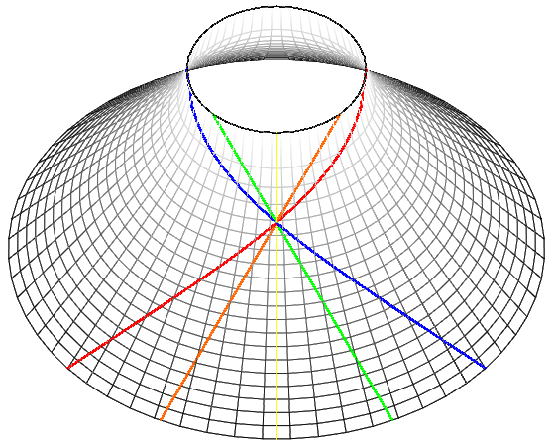
\includegraphics[height=2.7in]{../resources/PhD_thesis/dS_comoving_univ_rest.png}
\caption{A cut of the substrate read as a universe: comoving worldlines and
their null structure on the real de~Sitter surface. The exact cosmology is a
symmetry-breaking slicing of the maximally symmetric object, not a separate
geometry. (2012 dissertation.)}\label{fig:comoving}
\end{figure}

\paragraph{Matter's one geometric home.} The break has a residue. Maximal
symmetry, exhausting the continuous isometry, leaves over exactly the
\emph{discrete} orientation parity $O(5,1)\setminus SO_0(5,1)$---the
$\mathbb{Z}_2$ that threads the mass-reflection, the graviton helicities, and
the chirality of the turning polarisation plane past the
wall~\cite{JanzenGroupoid,JanzenDynamics,JanzenAlgebroid,JanzenBoundary}.
That discrete residue is the structurally indicated home of a fermion
sector, if the geometry carries one at all: not the continuous isometry the
wall closes, but the discrete parity the wall cannot reach. \textbf{[reach
--- do-not-assert, both ways; the ordinary route (a matter bundle placed by
hand) is untouched by the wall.]}

\paragraph{The generation conjecture, and the within-CR result it became.} One reach on that residue is worth
stating whole, as the conjecture it is, because its parts are grounded in
several registers at once and only the last step is open---and capturing it
coherently is how the corpus takes hold of a broad, tenuous structure to study
it. \textbf{Conjecture \textnormal{(do-not-assert).}} \emph{The Standard
Model's three fermion generations are the substrate's own three-fold slicing
structure, read on a spinor sector}---the three mass-tied roots of the one
$R$-odd offset-mass cubic (the $A_2$ weights), equivalently the three
$120^\circ$-separated hinged vantages of the one sliced substrate, carrying the
chirality $\gamma^5=R$. What is \emph{grounded}, in three registers:
\begin{itemize}
\item \emph{Geometry, the multiplicity.} The count is forced to three: the
offset-mass relation is the pure triple-angle $2M=\tfrac{2}{3\sqrt3}\sin 3w$,
driven to a single harmonic only at the unique slicing scale $2/\sqrt3$ the
gnomonic image of the hole fixes, so the three roots are the three preimages of
$3w$~\cite{JanzenSlicing}. Not fitted---forced.
\item \emph{Representation theory, the kind.} Of the residue's full
$D_6=S_3\times\mathbb{Z}_2$, only the $\mathbb{Z}_2$ is a substrate isometry
(the parity $R$, acting on the cut spinor as $\gamma^5$), so chirality descends
\emph{gauged}; the $S_3$ is the deck (Weyl) symmetry of the solution space and
no isometry ($\mathfrak{su}(3)\not\subset\mathfrak{so}(5,1)$), so a family
symmetry is \emph{global}---the Standard Model's own arrangement, gauged
chirality and global flavour, not assumed but following from which factor is an
isometry~\cite{JanzenBoundary,JanzenAlgebroid,JanzenGroupoid}.~The audit behind this count, its receipts, and the splits that cut its law are collected in the programme's combinatorics ledger (\texttt{COMBINATORICS\_LEDGER.md}).
\item \emph{Geometry again, the family as vantage.} The $S_3$ is realised
concretely as three $120^\circ$-separated hinged vantages: shifting the sky
angle by $2\pi/3$ fixes $2M$ and cycles the designated root through all three
(the cyclic $\mathbb{Z}_3$), $\sigma$ swapping the other two within a
hinge---three readings of the one substrate, converging from the geometry with
the representation-theoretic verdict that the family factor is a description
structure, not field copies~\cite{JanzenSlicing}.
\end{itemize}
The breaking is the slicing's own (the $r_0$-singling $2+1$ factorisation), the
mass \emph{values} the ordinary route. \textbf{The one open step---the
conjecture proper---is the descent:} whether a spinor sector
inherits this three-fold count, that is, whether three \emph{vantages} of the
one substrate are the three physical \emph{generations} a single observer sees.
That construction is built~\cite{JanzenMatter}: a spinor on the slicing structure binds exactly one chiral zero-mode at each throat wall \emph{as a bound mode of the existent leaf} (normalizable in the leaf's proper measure, where the propagating Dirac-norm mode does not)---its chirality the parity $R=\gamma^5$---and the maximally-symmetric matter construction, the one this programme's own principle selects over any single-hinge truncation (which would carry an unfixed arbitrary modulus), places a wall at each of the three hinges. The count is three, and the $S_3$ permuting the walls is the family symmetry. For the \emph{discrete flavour structure}---the generation count, the chirality, and the family symmetry---the physical identification is therefore a result, forced \emph{within} CR: it rests on the maximal-symmetry principle that defines the programme and on the fermion sector being set by the matter construction, which the wall calculation makes concrete, and on nothing further. What stays open beyond the discrete skeleton is the full \emph{propagating} spinor field sector (the built modes being leaf-bound, not the propagating theory); what stays the ordinary route is the gauge content (walled~\cite{JanzenBoundary}) and the mass spectrum (electroweak). Bold in shape, and, for the discrete skeleton, a result rather than a conjecture.

\paragraph{One principle, worn three ways.} Step back from the descent to the shape of the whole. The three-fold built there~\cite{JanzenMatter} is the innermost of three nested registers of maximal symmetry the construction carries. The substrate is maximally symmetric---$\mathrm{dS}_5$, its isometry $SO(5,1)$ exhausted (Prop.~\ref{prop:unique}). The evolving three-space it presents is maximally symmetric---the closed $S^3$ of the $\cosh$-law cosmology, $SO(4)$~\cite{JanzenOperator,JanzenCRcosmology}. And the discrete symmetry the slicing breaks out of the substrate is itself maximally symmetric---the hexagonal $\mathrm{Aut}(A_2)=D_6$, the $\mathbf 3\oplus\bar{\mathbf 3}$ worn on the two horns, the fundamental $\mathbf 3$ matter and its $R$-image $\bar{\mathbf 3}$ antimatter, at one weight within CR~\cite{JanzenMatter,JanzenBoundary}. Read this way the candidate synthesis widens past the generations: the Standard Model's apparent arbitrariness---why three families, why a chirality, why any discrete family structure at all---is, with the descent built~\cite{JanzenMatter} and forced within CR, not a list of inputs but the shadow of one principle broken symmetrically: a maximally-symmetric breaking of a maximally-symmetric substrate, carried in a maximally-symmetric space. The grounded floor is the three registers, and the discrete structure they carry is counted and built~\cite{JanzenMatter}, not conjectured: three chiral families related by $S_3$, forced within CR. What is \emph{not} claimed---and stays the ordinary route---is a geometric origin for the gauge content or the masses; those are walled and electroweak. For its discrete flavour skeleton, then, this is the thing the one principle reaches---within CR, at the weight the matter paper states in full.

\paragraph{The two readings: general relativity and the Standard Model's flavour, one discrete structure.} Stated at its sharpest, the synthesis is one claim about one discrete structure read two ways. The residue $\mathrm{Aut}(A_2)=S_3\times\mathbb{Z}_2\cong D_6$, read as \emph{cuts} of the substrate, is the organising symmetry of general relativity's symmetry-reducible solution space~\cite{JanzenRange}---the three horizon roots, the vantages that permute them, the mass-reflection $R$, the two null rulings; read on a \emph{fermion sector} it is the Standard Model's discrete flavour skeleton---a threeness against two chiralities, an $S_3$ and the parity $\gamma^5=R$~\cite{JanzenMatter}. \emph{The matter sector distinguishes two threes here and this paper follows it}: the $S_3$ among these vantages is the \emph{within-state} index, and the generations' threeness is the turnaround's deck $\mathbb{Z}_3$ (\emph{ibid.}). One structure, two readings, one slicing operator: the vacuum sector and the flavour skeleton are not two theories to be reconciled but two perspectival shadows of the one substrate's discrete symmetry---the reading, not the read, in the exact sense of \S\ref{sec:shadows}. Two boundaries hold this at its weight, and both are load-bearing rather than caveats. \emph{What the two readings share is the discrete residue, not the continuous symmetry:} the continuous isometry $SO(5,1)$ generates the cuts and is walled from the Standard Model ($\mathfrak{su}(3)\not\subset\mathfrak{so}(5,1)$~\cite{JanzenBoundary}), so it is the residue the exhausted continuous isometry leaves that both readings share, the gravitational reading keeping the continuous part to itself. \emph{And it is the flavour skeleton, not the gauge structure:} the Standard Model's defining $\mathrm{SU}(3)\times\mathrm{SU}(2)\times\mathrm{U}(1)$ is exactly the part \emph{not} read off the substrate (walled~\cite{JanzenBoundary}), the mass spectrum stays electroweak, and the reading delivers the generation count, the chirality, and the family symmetry and those alone. Nor does the synthesis unify the quantum with gravity: what the two readings share is a discrete \emph{geometric} symmetry, neither quantum nor classical in itself, while ``the quantum'' enters the corpus separately, in the horizon-thermal register of the ledger ($\hbar$ the Gibbons--Hawking gauge, \S\ref{sec:ledger})---so the old divide this synthesis bears on is between general relativity and the Standard Model's discrete content, not between general relativity and the quantum. A gravitational--cosmological unification whose matter reach is the discrete flavour skeleton, asserted nowhere as more. \textbf{[the crystallisation of \S\ref{sec:shadows} at its sharpest; the parts are established across the corpus~\cite{JanzenSlicing,JanzenGroupoid,JanzenOperator,JanzenDynamics}, the two-reading statement their consolidation, at coherence weight and do-not-assert on the world-correspondence.]}

% =====================================================================
\section{The space the corpus lands in}\label{sec:landing}
% =====================================================================

This section was opened as a stub by design and is now filled --- the two-way landing map below, complete across all sixteen rounds. The paper is opened so that the
propagation of the geometric core through the corpus fills it---and so that
the papers' consolidated cores back-propagate here, into one place, where
their deepest connections can land. The intended two-way flow:

\begin{itemize}
\item \textbf{P1, the metric singularity~\cite{JanzenBHcausality}} ---
\emph{round complete, both ways.} Forward: P1's scope note now points here, reading
its metric-singularity boundary as the structural forcing on which the
substrate's everywhere-real boundary rests (P1 standing on general relativity
alone, needing none of the substrate ontology). Reciprocal, into
\S\ref{sec:imaginary} and the augmentation rung of \S\ref{sec:unification}:
P1 supplies the \emph{structural} forcing complementary to P4's empirical one
--- the event horizon is a \emph{metric singularity} (a null hypersurface
along whose generators the spatial extent also contracts to zero), occurring
only as the null future boundary approached at infinite exterior time, so the
layered, cosmically-timed ontology the augmentation reads is forced
structurally as well as measured. It is the finite-curvature species of the
boundary genus (the infinite-curvature species and the genus in P2), the real
boundary of \S\ref{sec:imaginary} at its first exemplar. The two forcings ---
structural (P1, from general relativity alone) and empirical (P4, measured)
--- are independent and co-equal, neither resting on the other.
\item \textbf{P2, the Schwarzschild circle~\cite{JanzenCircle}} ---
\emph{round complete, both ways.} Forward: P2's introduction now points here, its
two-species genus and perspectival curvature the foundational-geometry
instance of the substrate's everywhere-real boundary and shadow-reading.
Reciprocal, into \S\ref{sec:imaginary} and \S\ref{sec:shadows}: P2 supplies
the \emph{genus} --- the event horizon and $r=0$ are the two $r$-poles of one
homogeneous circle, metric singularities of one genus differing only at second
order (curvature), so P1's finite-curvature species and the conjugate
infinite-curvature species are one object; and the curvature divergence at
$r=0$ is the curvature of the \emph{perspectival} metric, real as that
metric's and reading the chart's labelling --- the first, sharpest instance of
the shadow-reading of \S\ref{sec:shadows} (a real feature of a
vantage-dependent description, built-and-real, not an artefact in the
pejorative sense). The everywhere-real continuation through the seam
(\S\ref{sec:imaginary}) is the circle's own analytic completion. Sbierski's inextendibility concerns the maximal analytic
Schwarzschild spacetime, the $\Lambda=0$ object this construction does not contain; on the substrate the
geometry runs through the locus the chart labels $r=0$, $C^\infty$ across it~\cite{JanzenCRframework}.
\item \textbf{P3, the slicing curve~\cite{JanzenSlicing}} --- \emph{round complete,
both ways; the one-circle edge drawn (r1137).} Forward: P3's substrate-and-cut section now carries the
substrate-level statements this paper owns --- the Lorentzian signature
intrinsic to the positive curvature, the straight null rulings its own
``ruling legs'' run along, and the equilateral-pseudo-sphere $c$--$\Lambda$
mechanism --- pointing here for the full development. Reciprocal, into this
paper: P3 supplies the \emph{worked instances} of the core --- its slicing
curve is the cut of \S\ref{sec:shadows} realised; its \texttt{prop:flip} and
conjugate branch are the seam instance of \S\ref{sec:imaginary} (the flip
confined to the 2-surface, the conjugate region a real branch of the one
Lorentzian substrate); its two-sweeps/vantage-swap and its
$\alpha$-invariant/$M$-perspectival result are the shadow-reading
(\S\ref{sec:shadows}) and the constant-locking (\S\ref{sec:standard}) at
their first concrete rung. What P3 still hands forward: the coupled operations it now collects and owns---the root-exchange $\sigma$ and the backward-radial reflection $R$, coupled across both regimes, generating the substrate's full discrete symmetry---are the geometric base this paper reads at substrate altitude (the orientation $\mathbb{Z}_2$ of \S\ref{sec:shadows} being the $R$-factor of that coupled whole, advanced group-theoretically by P5); and the overcritical/lap
conjugacy is the geometric base of the phase-structure-at-the-seam
\textnormal{[reach: read at substrate altitude, with the geometric base established and the reading itself carried as a target, not a result]} (\S\ref{sec:frontiers}).
\item \textbf{P4, the modern parallax~\cite{JanzenModernParallax}} --- \emph{round
complete, both ways.} Forward: P4's exclusion section now points here, reading the
augmentation it forces as the empirical rung of the substrate's maximal
symmetry (carrying its own Copernican scope). Reciprocal, into
\S\ref{sec:unification} (the first and fifth rungs): P4 supplies the
\emph{empirical} rung --- the redshift-isotropy floor (accumulated-redshift
scatter $\sim10^{-3}$ against an observed $\lesssim3\times10^{-6}$, a
three-order exclusion) forces the cosmic foliation as a \emph{measured}
feature, and \texttt{thm:augmentation} establishes CR as the \emph{necessary
and sufficient} augmentation of general relativity for a description of an
existing, evolving world (the lapse the objective rate of advance, the shift
the relativity of synchrony). So the necessity of the first rung is not
posited but \emph{measured} --- the empirical counterpart of P1's structural
forcing, which stands on causal structure alone and needs none of this
evidence. Under the Copernican principle the same datum reaches the maximal
symmetry of the slices (the fifth rung, universality as the invariance of the
measure), which P4 marks as an \emph{extrapolation} beyond the directly
constrained region --- a scope \S\ref{sec:unification} inherits, not softens.
\item \textbf{P5, the description groupoid~\cite{JanzenGroupoid}} ---
\emph{round complete, both ways.} Forward: P5's \texttt{rem:orientation}
now reads its orientation-parity $\mathbb{Z}_2$ through this paper's lens ---
the discrete residue the exhausted continuous isometry leaves unspent, and
(do-not-assert) the structurally indicated matter home --- pointing here.
Reciprocal, into \S\ref{sec:shadows}: P5 supplies the residue's concrete
realisation --- the $\mathbb{Z}_2$ is the SdS solution space's own
$\mathrm{Aut}(A_2)=S_3\times\mathbb{Z}_2\cong D_6$---the coupled operations the slicing paper owns, advanced here into their group-theoretic form---the mass-reflection
$2M\mapsto-2M$ realised as the reticle reflection on the horizon-cubic roots
(\texttt{rem:orientation}), and the su(3)-guard from the gravitational side
(\texttt{rem:a2-distinct}: this $A_2$ is su(3)'s abstract root system in a
\emph{different realisation}, no colour via a continuous isometry --- whether
the shared abstract type is significant left open). The discrete residue of
\S\ref{sec:shadows} is thus not an abstraction but a worked group acting on
a concrete family.
\item \textbf{P6, the shadow of existence~\cite{JanzenShadowExistence}} ---
\emph{round complete, both ways.} Forward: P6 now points here (from its
closing placement in the programme), its theory-choice discipline the
epistemic ground on which this paper's
[reach] unification is held. Reciprocal, and it fixes the \emph{altitude} of
the whole paper: P6 supplies the \emph{epistemic engine} --- the
shadow-reading (infer the world that casts the appearances) of
\S\ref{sec:shadows}, the four rules with \emph{require over permit} (Rule~2)
the load-bearing one, the modal fallacy, and the constructive ordering
(ontology from evidence) --- and, above all, the boundary
\emph{self-consistency is not soundness}: the unification of
\S\ref{sec:unification} is a rule-favoured structure, and reading its several
established rungs as one fact is a theory-choice held at exactly that weight
(coherence, not correspondence), decidable by the test of
\S\ref{sec:frontiers}, its ultimate soundness the empirical question P6 sets
as the discipline's first programme. The \textbf{[reach]} tags throughout are
P6's discipline made explicit.
\item \textbf{P7, the framework~\cite{JanzenCRframework}} --- \emph{round
complete, both ways.} Forward: P7's null-boundary-correspondence section cites this paper for the
intrinsic-Lorentzian result and the $c$--$\Lambda$ mechanism, and its synthesis section now
points here for the maximal-symmetry reading that gathers its structural
recoveries. Reciprocal, and it is the deepest of the rounds: P7 supplies the
\emph{established} rungs of \S\ref{sec:unification} and the discipline that
holds them. Its central theorem (\texttt{thm:augmentation-p7},
\texttt{thm:cosmogenesis}) is the necessity-and-sufficiency rung as a formal
result; its synthesis reads three standing features of general relativity as
one substrate's --- the Carter constant~\cite{Carter1968} \emph{as the substrate's own maximal
symmetry surfacing}, the problem of time dissolved, the Dirac constraint
algebra as the symmetric-space grading $[\mathfrak{m},\mathfrak{m}]\subset
\mathfrak{h}$ of $SO(5,1)/SO(4,1)$ --- which is the maximal-symmetry
unification already at work at the structural rung. Above all, P7's synthesis section is
the altitude discipline this paper's \S\ref{sec:unification} must hold: the
closure of general relativity's solution space on one substrate is ``a
strong structural fact about the framework's internal economy; it is not,
and is not offered as, evidence that the world is so built,'' held to the two
open tests, self-consistency not soundness. The unification here is
\textbf{[reach]} at exactly that weight --- coherence, not correspondence ---
and P7's synthesis section is where the corpus states the discipline in full.
\item \textbf{P8, the slicing operator~\cite{JanzenOperator}} ---
\emph{round complete, both ways.} Forward: P8's introduction now points here, its
covariance-of-geometries substrate the geometric core's substrate.
Reciprocal, into \S\ref{sec:real} and \S\ref{sec:shadows}: P8 supplies the
\emph{operator} that realizes the substrate's cuts --- the slicing curve
promoted from classifier to a generating operator for the whole static
spherically-symmetric sector, with two derivations at the heart of the core's
picture: \emph{straight cuts are vacuum} (the SdS family is exactly the kernel
of the matter functional) and \emph{matter is the bend of the cut}
($\rho=m'/4\pi r^2$, the curvature of the cut off the vacuum profile). The
covariance is lifted one level --- the de Sitter substrate held invariant
under change of \emph{geometry} as general relativity holds one geometry
invariant under change of chart, ``many geometries, one substrate'' --- the
operational form of \S\ref{sec:real}; the reading grounded on the results, not
entailed by them (P6).
\item \textbf{P9, the range~\cite{JanzenRange}} --- \emph{round complete,
both ways.} Forward: P9's introduction now points here, its range the reach of the
substrate's maximal symmetry. Reciprocal, into \S\ref{sec:unification} and
\S\ref{sec:shadows}: P9 supplies the \emph{reach} of the construction --- the
range of the slicing operator is exactly the symmetry-reducible sector of
general relativity (every reachable geometry carries a sweep-subgroup of
$SO(5,1)$), filled across all Petrov types~\cite{Petrov1954}, so what the substrate's maximal
symmetry reaches is the constrained, non-radiative skeleton of general
relativity; the \emph{wall} is where continuous symmetry is lost --- genuinely
inhomogeneous matter, the onset of free gravitational radiation --- the
matter-boundary face (P13) read from the range side. And the Carter constant
general relativity carries as an unexplained gift is \emph{the substrate's
maximal symmetry surfacing} in the separable corner, one of the
maximal-symmetry recoveries the unification gathers (with P7). The reachable
catalogue is one substrate read through a vantage groupoid over a moduli
family of cuts.
\item \textbf{P10, canonical time~\cite{JanzenCanonicalTime}} --- \emph{round
complete, both ways.} Forward: P10 now points here (from its dissolution section),
its dissolution of the problem of time the canonical face of the substrate's
maximal symmetry. Reciprocal, into \S\ref{sec:unification} (the algebroid
rung): P10 is the \emph{canonical} complement to P12's structural account of
the problem of time --- where P12 identifies the obstruction (the
``wrong-sign'' structure function \emph{is} the substrate's coset metric, its
base-dependence the obstruction), P10 supplies the \emph{resolution}:
selecting the cosmic foliation the augmentation forces (empirically by the CMB
[P4], structurally by the horizon [P1]) deparametrizes the frozen constraint
into a \emph{true Hamiltonian}, the frozen and evolving readings the same
canonical content differing only in whether the manifold is granted existence
--- so the problem of time is \emph{dissolved}, not solved, by the same
ontological correction the whole augmentation makes. The closed-$S^3$ graviton
tower deparametrizes to unitary cosmic-time evolution and projects to the
flat-$\Lambda$CDM graviton, matter the bend of the slicing, not ontological
content.
\item \textbf{P11, why the cut bends~\cite{JanzenDynamics}} --- \emph{round
complete, both ways.} Forward: P11's chirality section now points here, the
graviton's handedness the radiating-sector face of the substrate's discrete
residue. Reciprocal, into \S\ref{sec:shadows} and the wall of
\S\ref{sec:unification}: P11 supplies the \emph{dynamics} --- why and how the
cut bends in time (the confined Gowdy--de Sitter wave, its energy and momentum
the shear of the leaf, deparametrized to P10's true Hamiltonian), located at
the Type-I edge, the last confined stratum before the \emph{wall} --- the
generative boundary (a Type-N plane wave, \emph{not} a metric singularity)
where generation-by-symmetry hands off to ordinary inhomogeneous evolution,
the dynamical face of P9's range boundary. And the chirality: past the wall
the graviton's two helicities settle a genuine handedness (the turning of the
polarization plane), the substrate's \emph{orientation parity} surfacing in
the radiating sector --- the disconnected $\mathbb{Z}_2$ of
\S\ref{sec:shadows}, beyond the index obstruction (P13), the dynamical face of
matter's one geometric residue. Cosmic no-hair makes the de Sitter background
an attractor; the continuous dynamics \emph{admits} rather than forces a
quantum structure, any forcing isolated to the discrete root structure (P12).
\item \textbf{P12, the constraint algebroid~\cite{JanzenAlgebroid}} ---
\emph{round complete, both ways.} Forward: P12's scope section now points here,
reading its symmetric-space recognition as one rung of the substrate's
maximal symmetry (at the coherence weight; its own result standing on the
symmetry-reducible sector). Reciprocal, into \S\ref{sec:unification} (the
sixth rung) and here: P12 supplies the \emph{deepest structural} rung ---
general relativity's own hypersurface-deformation (Dirac) algebra \emph{is}
the symmetric-space grading $[\mathfrak{m},\mathfrak{m}]\subset\mathfrak{h}$
of $SO(5,1)/SO(4,1)$ (\texttt{prop:closure}, term for term), and the
``wrong-sign'' structure function at the root of the problem of time
\emph{is} the substrate's Lorentzian coset metric, its base-dependence the
obstruction --- so the problem of time dissolves into a single geometric
fact of the maximal symmetry, established on the symmetry-reducible sector.
The orientation-parity $\mathbb{Z}_2$ of \S\ref{sec:shadows} is realised here
as the central inversion / double-ruling swap, and the su(3)-wall carried at
its careful do-not-assert ($SU(3)\not\subset SO(5)$; the $A_2$ the discrete
Weyl shadow only, no continuous colour isometry).
\item \textbf{P13, the matter boundary~\cite{JanzenBoundary}} --- \emph{round
complete, both ways.} Forward: P13's closing programme-significance section now points here, reading its wall as
one face of the substrate's maximal symmetry. Reciprocal, into
\S\ref{sec:unification} (the fourth rung) and \S\ref{sec:shadows}: P13
supplies the \emph{matter-boundary} rung --- the continuous matter symmetry
is walled because $SO(5,1)$ is \emph{complete} ($\mathfrak{su}(3)\not\subset
\mathfrak{so}(5,1)$; the geometric-isometry route closed four ways --- the
$\sigma$-lift a real Weyl reflection not the Wick rotation, the cascade
dropping the gauge at the real cut, the $A_2$ skeleton discrete-only, and the
Atiyah--Hirzebruch index rendering a compact-face fermion sector
vector-like), so the exhausted symmetry that locks the constants leaves no
room for a geometric colour. The mechanism is \emph{complementary}: the index
acts on the connected gauge group, the gravitational chirality on the
discrete orientation parity $\mathrm{O}(5,1)\setminus\mathrm{SO}_0$ the index
cannot reach, so observed fermion chirality is \emph{forced} non-geometric
--- and that same discrete parity is the discrete residue of
\S\ref{sec:shadows}, the single geometric opening the wall leaves
\textbf{[Reach, held do-not-assert: the structure is established; the reading of it offered here is not asserted by the corpus.]} The compact (Wick) face is
real-by-construction but, atemporal, no co-equal existent, by CR's
existence criterion.
\item \textbf{P14, the fermion sector~\cite{JanzenMatter}} --- \emph{round complete,
both ways; the one-circle edge drawn (r1137).} Forward: P14 points here, reading its three chiral
generations as the innermost of the three registers of maximal symmetry ---
the maximally-symmetric \emph{discrete} breaking the slicing takes from the
substrate. Reciprocal, into \S\ref{sec:shadows} and the matter rung of
\S\ref{sec:unification}: P14 supplies the \emph{built} discrete residue ---
the boundary's single geometric opening realised, three chiral families
related by a global $S_3$ with $R=\gamma^5$ chirality, forced within CR as the
maximally-symmetric slicing of a maximally-symmetric substrate, the gauge and
mass content external. The count is the substrate's discrete symmetry worn as
matter, originating at the $S_3$-fixed Nariai crest and unfolding as the
universe expands; whether it coheres with the empirical Standard Model stays
the data's to judge.
\item \textbf{P15, the cosmology~\cite{JanzenCRcosmology}} --- \emph{round
complete, both ways.} Forward: P15's introduction points here for the everywhere-real
substrate-and-boundary ontology, and its discussion for the root of its rigidity ---
$\Lambda$ the maximally symmetric substrate's sole scale. Reciprocal, into
\S\ref{sec:unification} (the third rung): P15 supplies the \emph{observational}
rung --- with $\Lambda$ the sole scale the cosmology carries no tunable
freedom (the parameter-free low-multipole deficit set by $\Lambda$ through
$r_0$ and $D_C$; the radiation-free rate; the transmission dichotomy --- no
inflationary scale-invariant attractor, no consistency relation, no
substrate-sourced $B$-modes), its discriminating power now
returned on the data --- the genuine-Boltzmann low-multipole shape a
cosmic-variance-limited wash (a smooth deficit bottoming at $\ell=4$,
neither the sharp observed quadrupole dip nor a sharp
falsification), while the radiation-free rate resolves the Hubble tension and
the primordial abundances return deuterium and helium within measurement on
the corpus's own hot dense history --- the one measured initial condition
$\rho_r/\rho_m$ an $\eta$-analogue read not tuned. The altitude discipline
still holds \S\ref{sec:unification} at coherence, but the observational rung
P15--P16 supply has since moved past it: on the discriminating axes the
cosmology has begun to earn correspondence, so that ``coherence shown is not
correspondence earned'' now marks the boundary between the structural
unification (held, still, at coherence) and the empirical confrontation (where
correspondence has started to be paid), not the whole programme's ceiling. The cosmic beginning is the
finite-curvature cosmogenesis branch point, reached through the conjugacy yet real.
\item \textbf{P16, the cosmogenesis~\cite{JanzenCosmogenesis}} --- \emph{round
complete, both ways.} Forward: P16 points here, reading the Big Bang as a
synthesis of the corpus's deductively forced consequences over this maximally
symmetric substrate --- the hot dense era the far side of a collapse the
substrate's own geometry already carries through the finite-curvature branch point.
Reciprocal, into \S\ref{sec:imaginary} and \S\ref{sec:shadows}: P16 lands the
\emph{lap} --- the conjugate branch of the slicing curve, reached through the
imaginary yet real, read forward as a previous universe's collapsed matter, the
\emph{cosmogenetic bead} the framework proves one closed curve~\cite{JanzenCRframework}
and a concrete instance of this paper's reached-through-the-imaginary principle
(its cosmic time runs off the real axis through a bounded contour while the areal
radius stays real at every point it lands on) ---
and returns the one quantitative consequence the synthesis adds beyond the
corpus's established results: the infalling matter, heated above the deuterium
bottleneck and re-expanded through it at the standard rate, runs a standard
nucleosynthesis that \emph{produces} the primordial light-element abundances
(helium-4 and deuterium at their observed values, the lithium problem shared
with $\Lambda$CDM). The Big Bang is thus no initial edge of the substrate but
a broken-symmetry shadow cast within it --- the substrate's maximal symmetry
read at the cosmogenesis rung, the abundances its fossil; its open edge whether
one progenitor handover fits all abundances together.
\end{itemize}

\noindent The discipline for filling this in is the corpus's own: reach to
the source, and let the connections the propagation reveals land here rather
than be forced. What this section will contain is not yet fully known; that
it will be filled by the two-way grind, and reveal structure the current
corpus does not name, is the working hypothesis under which the paper is
opened. \textbf{[reach --- the programme of the paper, stated for reversal.]}

% =====================================================================
\section{Frontiers}\label{sec:frontiers}
% =====================================================================

\begin{enumerate}
%  r2378 REGISTER ALIAS (observer line, ARC 14 step 2): the free-data-count test -- register `L-200`.
%  This list stays in the paper's own voice; the alias lives in a comment so a reader meets
%  the physics and a node can still trace what is owed.  Unregistered before r2378.
\item \textbf{The free-data-count test of the unification.} Show that the
framework's count of genuinely free data equals the substrate's
non-symmetric residue---maximal symmetry, spent, leaving exactly the one
measured cosmological IC ($\rho_r/\rho_m$) as the sole tunable datum, and
each constant-relation a locked parameter. Decisive: a hidden geometric
freedom in the cosmology, or a genuinely free constant where the reading
says it should lock, falsifies ``rigidity and wall are one fact.''
\textbf{[Reach: the item has two sides and they now stand differently, so it
is split rather than carried whole.]} \emph{The CONSTANT side is a result and
this paper carries it}: \S\ref{sec:ledger} states that the
gravitational--cosmological--quantum sector spends \emph{no free dimensionless
constant}, and the reason is structural rather than counted---neither real form
supplies a second invariant and a dimensionless magnitude needs
two\rcpt{P17_no_second_scale_on_either_face}, so there is a single dimensionful
input and nothing for a dimensionless tuning to hide in. \emph{And the
falsifier's second clause was met rather than asserted}: a place where a
genuinely free constant could have lived was checked and it locked---the metric
function, for a time the one input the construction did not derive, follows
entirely from $T^{t}{}_{t}=0$, a first-order linear equation whose whole
solution space is the Tangherlini--de~Sitter family with $M$ the single constant
of integration~\cite{JanzenSlicing}, obtained rather than
assumed\rcpt{P03_operator_at_general_D}. \emph{The DATUM side remains a
target}, and it is a different kind of quantity: $\rho_r/\rho_m$ is a matter
initial condition and not a constant, so it is not in the geometric residue at
all, and the programme calls it a one-parameter accommodation. \emph{And what was written here as owed is a
result, which is a different thing}\rcpt{X1_the_ratio_is_a_clock_reading_not_a_carried_datum}: the derivation from the progenitor
collapse cannot be delivered, for a structural reason rather than for want of
work. Radiation dilutes as $a^{-4}$ and matter as $a^{-3}$, so
$\rho_r/\rho_m\propto1/a$---\emph{a quantity that changes along the leg has no
single value for a handover to transmit}, and the progenitor's value at its own
maximum is a reading taken at one point on a curve. Nor does the crossing supply
one: a factor multiplying both components alike leaves the ratio unchanged, and
only a species-resolved factor could rescale it---which is exactly the rule
withdrawn when the crossing was shown lossless for every
species~\cite{JanzenCRframework}. \emph{So $\rho_r/\rho_m$ is where the
observable leg's own clock is read}, and a clock's zero is not the sort of thing
a handover carries. \emph{A frontier closed by impossibility is a finding and
this list should say so}: what is owed here is not a derivation but the
statement, now made, that there is none to give. \emph{And the companion
cosmogenesis paper reaches the same line from the other side, on a different
ground}: what a handover carries is what a conservation law protects, so $\eta$
crosses the compression peak because baryon number is conserved through it,
while the progenitor's composition is erased there because nuclear binding is
not---``two kinds of thing,'' in that paper's
words~\cite{JanzenCosmogenesis}. \emph{Two independent reasons, agreeing}: the
ratio is not carried because it is not constant along either leg, and it is not
carried because the crossing destroys what would have fixed
it.\rcpt{P17_the_frontier_item_is_a_result_and_the_cosmogenesis_paper_reaches_it_the_other_way}
%  r2376+c54.179: item 1 SPLIT.  Routed as FOR_54 item 15 by the observer line, and VERIFIED HERE against
%  this paper's own text rather than against the routed quotation -- which cites a budget sentence ("one
%  generator larger than the substrate's isometry group") that lives in that line's CORPUS_MAP and
%  DISSOLUTION_CENSUS and NOT in this paper.  The substance is nevertheless here, in this paper's voice and
%  with its own receipt: sec:ledger's "spending no free dimensionless constant" and the single-scale
%  argument at P17_no_second_scale_on_either_face; P3 supplies the met falsifier.  The split is the fork's,
%  as changing a paper's verdict on its own frontier must be.
%  r2378 REGISTER ALIAS (observer line, ARC 14 step 2): the maximal-symmetry ledger -- register `L-201`.
%  This list stays in the paper's own voice; the alias lives in a comment so a reader meets
%  the physics and a node can still trace what is owed.  Unregistered before r2378.
\item \textbf{The maximal-symmetry ledger.} Systematically determine what
geometric relations among the fundamental constants the substrate forces
($c$--$\Lambda$ and Nariai the two known instances), reading each as a spent
parameter; and look for any constant maximal symmetry does not reach---the
constant-side analogue of the discrete-parity matter opening. \textbf{[reach
--- grounded in two proven instances.]}
%  r2378 REGISTER ALIAS (observer line, ARC 14 step 2): the phase structure at the seam -- register `L-202`.
%  This list stays in the paper's own voice; the alias lives in a comment so a reader meets
%  the physics and a node can still trace what is owed.  Unregistered before r2378.
\item \textbf{The phase structure at the seam.} The everywhere-real claim is
established for the substrate and the seam as a geometric object; the
hypothesised phase structure at the seam relative to trajectories is the
interpretive layer the conjugacy programme opens, its geometric base real
and its trajectory/phase reading open. Decide whether it is real structure
or interpretation. \textbf{[reach --- held do-not-assert, both ways.]}
\end{enumerate}

\clearpage
\section*{Appendix R\quad Computational Receipts}\label{app:receipts}
\addcontentsline{toc}{section}{Appendix R: Computational Receipts}
\small\noindent Each computation marked \rcptmarker\ in the text is verified by a runnable receipt in the \texttt{receipts/} directory that ships with this work; status \textsf{OK} = verified (traced, run, output matches the claim). This appendix is generated from the receipt index, not maintained by hand.\par\medskip
\begingroup\renewcommand{\arraystretch}{1.25}
\begin{description}
\item[\label{rcpt:P17_the_alpha_family_is_a_foliation}\texttt{P17\_the\_alpha\_family\_is\_a\_foliation}]\hfill\textsf{[OK]}\\
\textit{the substrate ontology / the c--Lambda null-ruling gauge} \ (THE ALPHA-FAMILY IS A FOLIATION OF THE AMBIENT BY THE LEVEL SETS OF ONE QUADRATIC FORM, WITH THE LIGHT CONE AS ITS SINGULAR MEMBER -- AND THE CONFOCAL ORTHOGONALITY THEOREM, WHICH A STANDING LEAD EXPECTED TO APPLY, IS VACUOUS HERE FOR A STRUCTURAL REASON. THE PREMISE IS CORRECT: in the EQUILATERAL case -- which is what this substrate is -- the confocal family IS the dilation family. ** BUT THE CLASSICAL THEOREM IS NOT 'CONFOCAL QUADRICS ARE ORTHOGONAL' FULL STOP: it is that through a generic point pass THREE members, one of each type, and THOSE meet pairwise orthogonally. The confocal equation is CUBIC in the parameter generically and LINEAR in the equilateral case -- asserted -- so exactly ONE member passes through any point and there is no second member for it to be orthogonal TO. The hypothesis fails, not the conclusion. ** The same fact without machinery: a point assigns ONE value to the form, so distinct-alpha substrates are DISJOINT and cannot meet at any angle. ** THE DEGENERATION, NAMED: equilateral is exactly the confocal family's degenerate case -- as the semi-axes come together the cubic loses two roots, the three types collapse, and the triply-orthogonal system collapses with them. So the theorem went unused for the BEST POSSIBLE REASON: this substrate sits at the one point of the confocal moduli space where it has no content. ** ** AND WHAT SURVIVES IS BETTER THAN THE THEOREM WOULD HAVE BEEN: the family is a foliation -- de Sitter above zero, THE LIGHT CONE at zero, the two-sheet hyperboloid below. Different-alpha substrates NEST, do not meet, and share ONE asymptote, which is the family's own degenerate member. **). 
\emph{Computes:} the equilateral reduction computed; the degree in the confocal parameter computed and asserted (3 generic, 1 equilateral); the three signature classes tabulated
 \emph{Bound:} ** AND THAT IS A REASON FOR THE c--Lambda NULL-RULING GAUGE'S alpha-INDEPENDENCE, FROM THE FAMILY RATHER THAN FROM THE GAUGE: the null structure is carried by the one leaf common to the whole family, so it cannot depend on which leaf one stands on. This paper already calls the cone 'the locked asymptote' without connecting it to the family it belongs to. AND ONE ROUTING THE LEAD DID NOT ASK FOR: the map between members is a DILATION, which is CONFORMAL and not an isometry, so the alpha-family is a CONFORMAL ORBIT and belongs in the conformal ledger rather than the quadric-geometry file where it was left -- an item filed under the machinery someone first reached for rather than the machinery that fits it **
\ \emph{Run:} \texttt{python3 receipts/P17\_geometric\_core\_paper/P17\_the\_alpha\_family\_is\_a\_foliation.py}
\item[\label{rcpt:P17_power_of_a_point}\texttt{P17\_power\_of\_a\_point}]\hfill\textsf{[OK]}\\
\textit{sec:power} \ (**!! c54.161: THE CIRCULARITY IS RETIRED** -- the power is now MEASURED from bisected secant products and compared against X0 taken from the substrate constraint, at 2 alpha and 3 alpha, so eq:powerisheight is no longer true by construction. **!! MARKED c54.157: THE CITING SENTENCE ATTRIBUTES TO THIS FILE FIGURES IT DOES NOT PRODUCE** -- the ds\textasciicircum{}2, the 600 random heights and the max 5.7e-14 all come from `P17\_power\_is\_null`. **And its own eq:powerisheight is circular: X0 is DEFINED as sqrt(\textbar{}X\textbar{}\textasciicircum{}2 - alpha\textasciicircum{}2), so 'power = X0\textasciicircum{}2' holds by construction.** What it does compute honestly is Euclid III.36 -- the secant invariance to 4.4e-16 over 500 sightlines. Original claim: power of a point pow(P)=\textbar{}X\textbar{}\textasciicircum{}2-alpha\textasciicircum{}2 (Steiner/Euclid III.36) = invariant: hinge power=3 exact; 500 random sightlines PX.PY=\textbar{}PO\textbar{}\textasciicircum{}2-alpha\textasciicircum{}2 to 4.4e-16). 
\emph{Computes:} every-sightline invariant test at machine precision
\ \emph{Run:} \texttt{python3 receipts/P17\_geometric\_core\_paper/P17\_power\_of\_a\_point.py}
\item[\label{rcpt:P17_power_is_null}\texttt{P17\_power\_is\_null}]\hfill\textsf{[OK]}\\
\textit{sec:power prop:tangentnull} \ (tangent to throat is NULL: tangent length=\textbar{}X0\textbar{}=sqrt(R\textasciicircum{}2-alpha\textasciicircum{}2) identity (Euclid=hyperboloid RHS); ds\textasciicircum{}2=-dX0\textasciicircum{}2+\textbar{}dX\textbar{}\textasciicircum{}2=0, max 5.68e-14 over 600 heights (=paper's 5.7e-14); power-of-a-point = null condition, same equation). 
\emph{Computes:} tangent-length identity + ds\textasciicircum{}2=0 at 600 random points
\ \emph{Run:} \texttt{python3 receipts/P17\_geometric\_core\_paper/P17\_power\_is\_null.py}
\item[\label{rcpt:P17_qm_S4_vs_S5}\texttt{P17\_qm\_S4\_vs\_S5}]\hfill\textsf{[OK]}\\
\textit{sec:ledger} \ (**!! CORRECTED c54.157: THE ROW CLAIMED THREE VERIFIED ITEMS AND ONE WAS VERIFIED.** The realified-generator antisymmetry is computed; **'minimal faithful real rep R\textasciicircum{}6' was a print string** (exhibiting one 6-dimensional rep shows su(3) FITS in so(6) and excludes nothing about 5), and 'GH beta = 2 pi alpha n-independent' has kappa hardcoded to 1.0 and never varies with n. **The minimality is now ENUMERATED by the Weyl dimension formula over su(3)'s irreps: the smallest faithful real dimension is 6, attained by 3 + 3-bar, so no faithful real rep fits in R\textasciicircum{}5.** Original claim: su(3) requires so(6)/S\textasciicircum{}5 not so(5)/S\textasciicircum{}4: 8 Gell-Mann generators realified to R\textasciicircum{}6 all antisymmetric (max\textbar{}R+R\textasciicircum{}T\textbar{}=0.0 -> so(6)), faithful on all 6 real dims (minimal real rep R\textasciicircum{}6); GH beta=2pi alpha n-independent -> thermal + gauge Euclideans co-locate on one real form (S\textasciicircum{}5 or S\textasciicircum{}4 equator)). 
\emph{Computes:} realified-generator antisymmetry + faithful-dimension + GH n-independence
\ \emph{Run:} \texttt{python3 receipts/P17\_geometric\_core\_paper/P17\_qm\_S4\_vs\_S5.py}
\item[\label{rcpt:C3_inversion_extends}\texttt{C3\_inversion\_extends}]\hfill\textsf{[OK]}\\
\textit{rem:onecircle} \ (C3 --- does INVERSION in the throat extend off the equatorial plane, as polarity did (Q1/Q6)? Minkowski inversion in the quadric eta(X,X)=alpha\textasciicircum{}2: P* = alpha\textasciicircum{}2 P / eta(P,P).). 
\emph{Computes:} runs clean; registered r2376 (c54) from its own docstring and a live run
 \emph{Bound:} description is the receipt's own wording, condensed; not independently re-derived here
\ \emph{Run:} \texttt{python3 receipts/P17\_geometric\_core\_paper/C3\_inversion\_extends.py}
\item[\label{rcpt:D1_hinge_duality}\texttt{D1\_hinge\_duality}]\hfill\textsf{[OK]}\\
\textit{rem:onecircle} \ (D1 --- PROJECTIVE DUALITY: the dual of the swinging door. PRIMAL : the pencil of slicing planes (doors) through the HINGE. DUALITY : in the plane of the throat, w.r.t. the throat circle \textbar{}x\textbar{}\textasciicircum{}2 = alpha\textasciicircum{}2, the pencil of LINES through a point P dualises to the RANGE OF POINTS on P's POLAR. So the dual of the swing is a POINT SLIDING ALONG THE HINGE'S POLAR. Where is that line?). 
\emph{Computes:} runs clean; registered r2376 (c54) from its own docstring and a live run
 \emph{Bound:} description is the receipt's own wording, condensed; not independently re-derived here
\ \emph{Run:} \texttt{python3 receipts/P17\_geometric\_core\_paper/D1\_hinge\_duality.py}
\item[\label{rcpt:D3_segre_no_pencil}\texttt{D3\_segre\_no\_pencil}]\hfill\textsf{[OK]}\\
\textit{rem:onecircle} \ (D3 --- SEGRE. The Segre symbol classifies a PENCIL of quadrics by the elementary divisors of lambda A + mu B. So the probe needs an honest answer to: DOES THE CORPUS HAVE TWO QUADRICS IN ONE SPACE? Confirmation 4, before anything runs. Candidates, each checked:). 
\emph{Computes:} runs clean; registered r2376 (c54) from its own docstring and a live run
 \emph{Bound:} description is the receipt's own wording, condensed; not independently re-derived here
\ \emph{Run:} \texttt{python3 receipts/P17\_geometric\_core\_paper/D3\_segre\_no\_pencil.py}
\item[\label{rcpt:O2_sightline_null_on_lift}\texttt{O2\_sightline\_null\_on\_lift}]\hfill\textsf{[OK]}\\
\textit{prop:tangentnull} \ (O2 --- p0's tangent/secant distinction, and whether it is a shadow boundary in the optics sense. p0: 'sightlines of the projection that TOUCH the throat are light rays; those that CUT it are not.'). 
\emph{Computes:} runs clean; registered r2376 (c54) from its own docstring and a live run
 \emph{Bound:} description is the receipt's own wording, condensed; not independently re-derived here
\ \emph{Run:} \texttt{python3 receipts/P17\_geometric\_core\_paper/O2\_sightline\_null\_on\_lift.py}
\item[\label{rcpt:Q1_quadric_polarity}\texttt{Q1\_quadric\_polarity}]\hfill\textsf{[OK]}\\
\textit{rem:onecircle} \ (Q1, invariant form. The first pass computed a EUCLIDEAN distance for the polar hyperplane in a MINKOWSKI space and got 1/sqrt7 = 0.37796 -- a gauge artifact, not an invariant. Redone with the only quantity polarity actually depends on: eta(P,P) against alpha\textasciicircum{}2.). 
\emph{Computes:} runs clean; registered r2376 (c54) from its own docstring and a live run
 \emph{Bound:} description is the receipt's own wording, condensed; not independently re-derived here
\ \emph{Run:} \texttt{python3 receipts/P17\_geometric\_core\_paper/Q1\_quadric\_polarity.py}
\item[\label{rcpt:Q3_cayley_klein}\texttt{Q3\_cayley\_klein}]\hfill\textsf{[OK]}\\
\textit{---} \ (Q3 --- Cayley-Klein: is the substrate's metric a log-cross-ratio against the absolute, and is alpha the CK scale constant? Substrate dS\_5 = \{X in M\textasciicircum{}6 : eta(X,X)=alpha\textasciicircum{}2\}.). 
\emph{Computes:} runs clean; registered r2376 (c54) from its own docstring and a live run
 \emph{Bound:} description is the receipt's own wording, condensed; not independently re-derived here
\ \emph{Run:} \texttt{python3 receipts/P17\_geometric\_core\_paper/Q3\_cayley\_klein.py}
\item[\label{rcpt:Q6r_polar_is_the_background}\texttt{Q6r\_polar\_is\_the\_background}]\hfill\textsf{[OK]}\\
\textit{---} \ (Q6-CONFIRMED --- the polar slice sits at RUNG 2, and that answers A18. CONFIRMATION 1 (ontology): section 0's five-rung ladder. Rung 1 = the substrate dS\_5 = SO(5,1)/SO(4,1). Rung 2 = 'A CUT of the substrate -- a four-geometry. dS\_4 is one such: the maximally symmetric one... A geometry is a cut exactly when its isometry group contains a sweep-subgroup of the substrate's.'). 
\emph{Computes:} runs clean; registered r2376 (c54) from its own docstring and a live run
 \emph{Bound:} description is the receipt's own wording, condensed; not independently re-derived here
\ \emph{Run:} \texttt{python3 receipts/P17\_geometric\_core\_paper/Q6r\_polar\_is\_the\_background.py}
\item[\label{rcpt:P17_no_second_scale_on_either_face}\texttt{P17\_no\_second\_scale\_on\_either\_face}]\hfill\textsf{[OK]}\\
\textit{the constant ledger} \ (**NEITHER REAL FORM OF THE SUBSTRATE SUPPLIES A SECOND SCALE, SO THE CONSTRUCTION CANNOT FORCE A DIMENSIONLESS MAGNITUDE. THE SILENCE IS A PROPERTY, NOT A GAP.** The Wick rotation X0 -> i X0 carries the defining quadric to S\textasciicircum{}5 of the SAME radius alpha -- it acts on the COORDINATE and leaves the right-hand side untouched, so no step exists at which a second radius could enter; the two faces are the two real forms of one complex quadric and a real form does not choose its own radius. Every curvature invariant on both faces is a pure power of 1/alpha\textasciicircum{}2 (asserted by logarithmic derivative), leaving no second constant with which to form a ratio. The remaining candidates are enumerated and each disposed: the horizon period is built from alpha; M and r\_0 are moduli; 2/(3 sqrt 3) is one member's value. **So a dimensionless magnitude cannot be forced, and that is the COMMON ROOT of three verdicts already banked separately -- the winding quantises and cannot measure, the flat bundle selects and cannot couple, the branch point filters and cannot supply.**). 
\emph{Computes:} the Wick image asserted equal to S\textasciicircum{}5 of radius alpha; each invariant's logarithmic derivative asserted an integer
 \emph{Bound:} **bound: this is about the two faces' GEOMETRY. Fields living on either face may carry their own scales -- but those are CONTENT, adjoined rather than derived, and adjoining one is what the corpus's admissibility criterion rejects. The escape exists and costs the thing the programme is for**
\ \emph{Run:} \texttt{python3 receipts/P17\_geometric\_core\_paper/P17\_no\_second\_scale\_on\_either\_face.py}
\item[\label{rcpt:P03_operator_at_general_D}\texttt{P03\_operator\_at\_general\_D}]\hfill\textsf{[OK]}\\
\textit{rem:dimension / thm:kernel} \ (** ASSUMPTION (A1) DISCHARGED. ** CR's OWN operator at general D returns Tangherlini-de Sitter and nothing else. The point previously missed: CR's operator is NOT a metric function -- P8 thm:kernel defines the vacuum sector as the KERNEL OF THE MATTER FUNCTIONAL on a cut in the construction gauge ('derived, not matched'), and that condition runs at any D. Computed from the metric rather than quoted: for ds\textasciicircum{}2 = -f dt\textasciicircum{}2 + dr\textasciicircum{}2/f + r\textasciicircum{}2 dOmega\textasciicircum{}2\_\{D-2\}, G\textasciicircum{}t\_t = (D-2)/(2r\textasciicircum{}2)[r f' + (D-3)(f-1)] (verified at D=4,5,6), so T=0 is the first-order linear ODE r f' + (D-3)(f-1) + 2 Lambda r\textasciicircum{}2/(D-2) = 0 -- P8's own equation at D=4 -- whose ENTIRE solution space at D=4,5,6,7,8 is f = 1 - 2M/r\textasciicircum{}(D-3) - 2 Lambda r\textasciicircum{}2/((D-1)(D-2)) with ONE constant of integration, verified identical to Tangherlini-dS at every D tested. With alpha(D) = sqrt((D-1)(D-2)/2Lambda), which returns sqrt(3/Lambda) at four, this is f = 1 - 2M/r\textasciicircum{}(D-3) - r\textasciicircum{}2/alpha\textasciicircum{}2 at every D, and the dimension result's input 2M = r\_0\textasciicircum{}(D-3) - r\_0\textasciicircum{}(D-1) is that f at a root. THE DIMENSION RESULT THEREFORE STRENGTHENS: the collapse, the fold being D-1 and the mass parity all run on a function the construction GENERATES rather than borrows [borrowed from P3 / P8]). 
\emph{Computes:} the Einstein tensor computed from the metric at D=4,5,6 and matched to the closed form; the ODE solved by dsolve at D=4..8 and compared term by term with Tangherlini-dS
 \emph{Bound:} TWO INPUTS REMAIN AND ARE NAMED: (i) THE LOCK -- the construction gauge g\_tt g\_rr = -1 is assumed at general D, and P8 says the single slicing curve enforces it at four but this does not show it does so at general D (L-89; P8's lapse split is the machinery that would say otherwise); (ii) THE SPHERE -- the transverse space is taken round S\textasciicircum{}\{D-2\}, which at general D is a choice (L-90). And (A2), the single-harmonic collapse being a REQUIREMENT at other D, is untouched
\ \emph{Run:} \texttt{python3 receipts/P03\_SdS\_slicing/P03\_operator\_at\_general\_D.py}
\item[\label{rcpt:P17_the_cut_is_planar_only_at_M_zero}\texttt{P17\_the\_cut\_is\_planar\_only\_at\_M\_zero}]\hfill\textsf{[OK]}\\
\textit{the ladder / sec:slicing / sec:pd} \ (**!! c54.161: THE TWO c54.157 MARKINGS ARE RETIRED** -- the hyperplane split is now done for a tilted n with the induced Ricci scalar computed as 12/(alpha\textasciicircum{}2-c\textasciicircum{}2), and the Kretschmann scalar is DERIVED from the metric rather than typed in. **!! CORRECTED c54.157: THE ROW'S 'the hyperplane split done in general' IS FOUR PRINT STATEMENTS AND A HARDCODED TABLE**, and the Kretschmann scalar 48M\textasciicircum{}2/r\textasciicircum{}6 + 24/alpha\textasciicircum{}4 is an INPUT typed at line 97, not a finding -- it is derived from the metric in `P07\_sds\_kretschmann`, which is where the paper should look. The remaining evidence items (the M-factored closure defect, the r-dependent kappa\textasciicircum{}2, the M = 0 control) are accurate. Original claim: WHAT "CUT" CAN MEAN, COMPUTED. EVERY HYPERPLANE SECTION OF dS\_5 HAS CONSTANT CURVATURE -- splitting X = c n + Y gives eta(Y,Y) = alpha\textasciicircum{}2 - c\textasciicircum{}2, a dS\_4 of radius sqrt(alpha\textasciicircum{}2-c\textasciicircum{}2), for every n and c; a quadric cut by a linear space is a quadric. And SdS has K = 48 M\textasciicircum{}2/r\textasciicircum{}6 + 24/alpha\textasciicircum{}4, non-constant unless M = 0. ** SO A PLANE SECTION OF dS\_5 IS SdS IF AND ONLY IF M = 0 ** -- which CONFIRMS p0's polar hyperplane and shows it is not one example but THE only one. HENCE MATTER MUST BEND THE CUT, now a theorem rather than a reading. AND THE BENT CUT DOES NOT CLOSE EITHER: with P3's own symmetry (round areal sphere in a spacelike 3-block, staticity as the ambient boost the pencil turns on), lying ON the substrate fixes G and inducing SdS fixes G' -- two determinations of one function, and solving for kappa\textasciicircum{}2 returns an r-DEPENDENT expression, contradicting kappa's definition. ** AND THE FORM OF THE OBSTRUCTION IS THE RESULT: the closure defect factors with an OVERALL FACTOR OF M. The failure of a cut to close as a hypersurface IS the mass it carries, linearly, with no other source ** [borrowed from P17 / P3 / P9]). 
\emph{Computes:} the hyperplane split done in general; the Kretschmann derivative; the two determinations of G' computed and subtracted; kappa\textasciicircum{}2 solved for and shown r-dependent; the M = 0 control returning residual 0 and G = 0 (the planar vacuum cut)
 \emph{Bound:} ** IT DOES NOT REFUTE THE CUT RELATION, and reading it that way would be the error the receipt exists to prevent: P9 defines a cut by its isometry group containing a sweep-subgroup, P12 by an orientation plus causal-vantage datum, and the framework calls SdS a DERIVATIVE metric, not an induced one. What is established is that the ISOMETRIC-EMBEDDING reading is available at M=0 and nowhere else, so the corpus owes a sentence saying which relation 'cut' names **
\ \emph{Run:} \texttt{python3 receipts/P17\_geometric\_core\_paper/P17\_the\_cut\_is\_planar\_only\_at\_M\_zero.py}
\item[\label{rcpt:P0_the_order_parameter_is_the_offset_and_it_is_bounded_by_the_nariai_member}\texttt{P0\_the\_order\_parameter\_is\_the\_offset\_and\_it\_is\_bounded\_by\_the\_nariai\_member}]\hfill\textsf{[OK]}\\
\textit{sec:residue} \ (**ITEM 48 WORKED: THE TWO SYMMETRY BREAKINGS ARE ONE OBJECT, AND JOINING THEM GIVES THE HIGGS IDENTIFICATION ACTUAL CONTENT.** Lead `L-521`; VEIN `L-221`. **PART 1** p0 states the parity as \$r\_0\textbackslash\{\}mapsto-r\_0\$ (whence \$2M\textbackslash\{\}mapsto-2M\$); P3 derives \$2M=r\_0-r\_0\textasciicircum{}3\$ for a different purpose; **the cubic is odd, so p0's mass-reflection is an IDENTITY of P3's relation** and the two breakings are one object. **PART 2** \$2M=0\$ at \$r\_0=0,\textbackslash\{\}pm\textbackslash\{\}alpha\$ with \$f=1-r\textasciicircum{}2/\textbackslash\{\}alpha\textasciicircum{}2\$ at all three --- **the symmetric sector is the bare substrate**, one geometry read at three offsets. **PART 3** over P3's admissible range \$\textbackslash\{\}lvert r\_0\textbackslash\{\}rvert\textbackslash\{\}le2\textbackslash\{\}alpha/\textbackslash\{\}sqrt3\$, **\$\textbackslash\{\}lvert M\textbackslash\{\}rvert\textbackslash\{\}le\textbackslash\{\}alpha/3\textbackslash\{\}sqrt3\$ --- the Nariai mass, derived independently from \$f=f'=0\$**; a quartic potential is unbounded in its field and this order parameter is not, saturating at the configuration a collapse reaches. **PART 4** eight source checks across p0 and P3, including that p0 now names the Higgs (zero uses in seventeen papers) and keeps `F1` explicit. [borrowed from p0]). 
\emph{Computes:} **the oddness of \$2M(r\_0)\$ --- this IS the join; if P3's relation were not odd, p0's mass-reflection would be a separate assumption and there would be no single object**; all three roots asserted to give the same de Sitter metric function, both as the symmetric-sector claim and so "three roots" cannot be read as three vacua; the bound asserted numerically over P3's own range AND identified with the Nariai mass **derived independently and never substituted in, because the whole content is that two separately-derived numbers coincide**; and eight source checks
 \emph{Bound:} **scope: a statement about the MECHANISM, which is what item 48 asked for. NOT claimed: any vacuum expectation value, electroweak scale or mass value; any derivation of the Higgs field, its potential or its gauge group. `F1` untouched and said so in the paper's own voice. And the three roots are three offsets on ONE geometry --- vantage multiplicity already in the corpus.**
\ \emph{Run:} \texttt{python3 receipts/P17\_geometric\_core\_paper/P0\_the\_order\_parameter\_is\_the\_offset\_and\_it\_is\_bounded\_by\_the\_nariai\_member.py}
\end{description}\endgroup


\begin{thebibliography}{99}
\bibitem{JanzenThesis} D.~Janzen, \emph{A Solution to the Cosmological
Problem of Relativity Theory} (PhD dissertation, University of Saskatchewan,
2012), ch.~3.

\bibitem{CoxeterGreitzer1967} H.~S.~M.~Coxeter and S.~L.~Greitzer, \emph{Geometry Revisited}, Mathematical Association of America, Washington DC (1967).
\bibitem{Coxeter1987b} H.~S.~M.~Coxeter, \emph{Projective Geometry}, 2nd ed., Springer, New York (1987).
\bibitem{Casey1866} J.~Casey, \emph{On the equations and properties of the circles of a triangle}, Proc.\ R.\ Irish Acad.\ \textbf{9} (1866) 396--423.
\bibitem{Cayley1859} A.~Cayley, \emph{A sixth memoir upon quantics}, Philos.\ Trans.\ R.\ Soc.\ Lond.\ \textbf{149} (1859) 61--90.
\bibitem{Klein1871} F.~Klein, \emph{\"Uber die sogenannte Nicht-Euklidische Geometrie}, Math.\ Ann.\ \textbf{4} (1871) 573--625.
\bibitem{Steiner1826} J.~Steiner, \emph{Einige geometrische Betrachtungen},
J. reine angew. Math. \textbf{1}, 161--184 (1826).

\bibitem{Euclid} Euclid, \emph{Elements}, Book~III, Prop.~36 (c.~300 BCE);
T.~L.~Heath (trans.), \emph{The Thirteen Books of Euclid's Elements}, 2nd ed.
(Cambridge University Press, 1926).
\bibitem{Eddington1923} A.~S.~Eddington, \emph{The Mathematical Theory of
Relativity} (Cambridge University Press, 1923), \S~66 (the interpretation of
Einstein's law of gravitation).
\bibitem{Eddington1933} A.~S.~Eddington, \emph{The Expanding Universe}
(Cambridge University Press, 1933).
\bibitem{Chandrasekhar1983} S.~Chandrasekhar, ``Eddington: the most
distinguished astrophysicist of his time'' (centenary lecture, 1983).
\bibitem{JanzenBHcausality} D.~Janzen, \emph{The event horizon is a metric singularity: a missing definition in general relativity}, companion paper (P1).
\bibitem{JanzenCircle} D.~Janzen, \emph{The Schwarzschild and de Sitter circle: the intrinsic geometry of one homogeneous ring---the event horizon and the curvature singularity at $r=0$ its two poles}, companion paper (P2).
\bibitem{JanzenSlicing} D.~Janzen, \emph{The de Sitter substrate and its slicing curve: horizons as turning points, and de Sitter and Schwarzschild as two readings of one slicing}, companion paper (P3).
\bibitem{JanzenGroupoid} D.~Janzen, \emph{The Schwarzschild--de Sitter description groupoid: generators, relations, and Schwarzschild as the asymmetric realisation}, companion paper (P5).
\bibitem{JanzenModernParallax} D.~Janzen, \emph{The modern parallax: the redshift-isotropy floor, the empirical forcing of cosmic time and uniform expansion, and the measured resolution of the relativity of simultaneity}, companion paper (P4).
\bibitem{JanzenShadowExistence} D.~Janzen, \emph{The shadow of existence: scientific theory-choice as an empirically grounded discipline, calibrated on the historical record}, companion paper (P6).
\bibitem{JanzenCRframework} D.~Janzen, \emph{Collapsed matter must become a universe: the necessary and sufficient augmentation of general relativity into a description of structural existence, proven for gravitational collapse of any symmetry}, companion paper (P7).
\bibitem{JanzenOperator} D.~Janzen, \emph{Covariance of geometries over the de Sitter substrate: the slicing operator, the vacuum kernel, and matter as the bend of the cut}, companion paper (P8).
\bibitem{JanzenRange} D.~Janzen, \emph{The range of the de Sitter slicing operator: surjectivity onto the symmetry-reducible sector of general relativity, the Kerr--NUT--(A)dS vacuum kernel, and the wall of inhomogeneity}, companion paper (P9).
\bibitem{JanzenCanonicalTime} D.~Janzen, \emph{The canonical problem of time as a category error: an empirically forced cosmic time, deparametrization, the dissolution of frozen dynamics, and a graviton quantization the de~Sitter horizon closes without a free parameter---the seam where $\hbar$ enters gravity---in Cosmological Relativity}, companion paper (P10).
\bibitem{JanzenDynamics} D.~Janzen, \emph{Why the cut bends: the dynamics of the de Sitter cut, the confined gravitational wave, the generative boundary of the slicing operator, and chirality as the turning of the polarization plane}, companion paper (P11).
\bibitem{JanzenAlgebroid} D.~Janzen, \emph{General relativity's constraint algebra as the symmetric-space structure of a de Sitter substrate: the action Lie algebroid of the symmetry-reducible sector, and the problem of time's ``wrong sign'' as the substrate's coset signature}, companion paper (P12).
\bibitem{JanzenCRcosmology} D.~Janzen, \emph{The cosmology of Cosmological Relativity: the expansion history from causal reassignment on a de~Sitter background, the cosmogenesis branch point, and the scalar perturbation sector}, companion paper (P15).
\bibitem{JanzenBoundary} D.~Janzen, \emph{The de Sitter substrate and the Standard Model: a four converging routes to a geometric boundary on what one maximally-symmetric Lorentzian substrate's isometry does and does not force, and the framework and gauge on its two real forms}, companion paper (P13).
\bibitem{JanzenCosmogenesis} D.~Janzen, \emph{Cosmogenesis: the Big Bang as a synthesis of Cosmological Relativity's deductively forced consequences, and the primordial light-element abundances it produces}, companion paper (P16).
\bibitem{JanzenMatter} D.~Janzen, \emph{The fermion sector of Cosmological Relativity: three chiral generations from the maximally-symmetric slicing structure}, companion paper (P14).
\bibitem{GibbonsHawking1977} G.~W.~Gibbons and S.~W.~Hawking, \emph{Cosmological event horizons, thermodynamics, and particle creation}, Phys.\ Rev.\ D \textbf{15} (1977) 2738.
\bibitem{Nariai1951} H.~Nariai, \emph{On a new cosmological solution of Einstein's field equations of gravitation}, Sci.\ Rep.\ T\^ohoku Univ.\ Ser.\ I \textbf{35} (1951) 62; reprinted in Gen.\ Rel.\ Grav.\ \textbf{31} (1999) 963.
\bibitem{Carter1968}
B.~Carter,
\emph{Global structure of the Kerr family of gravitational fields},
Phys.~Rev.~\textbf{174} (1968) 1559--1571.
\bibitem{Petrov1954}
A.~Z.~Petrov,
\emph{The classification of spaces defining gravitational fields},
Uchenye Zapiski Kazanskogo Universiteta \textbf{114}, 55 (1954); reprinted in Gen. Rel. Grav. \textbf{32}, 1665 (2000).
\end{thebibliography}

\end{document}
